% !TeX program = pdflatex
\documentclass[12pt,a4paper]{article}

% =====================================================================
%  PACOTES ESSENCIAIS
% =====================================================================
\usepackage[brazilian]{babel}
\usepackage[utf8]{inputenc}
\usepackage[T1]{fontenc}
\usepackage{lmodern}
\usepackage{graphicx}
% prefixo figures/ explicitamente, evitando redundância de caminho.
\usepackage{cite}
\usepackage{amsmath}
\usepackage{amssymb}
\usepackage{indentfirst}
\usepackage{geometry}
\usepackage{booktabs}
\usepackage{multirow}
\usepackage{array}
\usepackage{subcaption}
\usepackage{float}
\usepackage{xcolor}
\usepackage{tikz}
\usepackage{tcolorbox}
\usepackage{fancyhdr}
\usepackage{titlesec}
\usepackage{enumitem}
\usepackage{microtype}
\microtypesetup{expansion=false}
\usepackage{url}
\usepackage{setspace}
\usepackage{caption}
\usepackage{siunitx}          % formatação consistente de unidades (dB, kHz, ms)
\DeclareSIUnit{\lufs}{LUFS}    % unidade de loudness usada no AGC
\usepackage{hyperref}         % sempre o ÚLTIMO pacote

% =====================================================================
%  ESPAÇAMENTO ABNT (NBR 14724:2011)
% =====================================================================
\onehalfspacing
\frenchspacing

% =====================================================================
%  CONFIGURACAO TIKZ
% =====================================================================
\usetikzlibrary{shapes.geometric, arrows, positioning, fit}

% =====================================================================
%  CORES
% =====================================================================
\definecolor{primaryblue}{RGB}{41, 128, 185}
\definecolor{accentblue}{RGB}{52, 152, 219}
\definecolor{successgreen}{RGB}{39, 174, 96}
\definecolor{warningorange}{RGB}{243, 156, 18}
\definecolor{dangerred}{RGB}{231, 76, 60}
\definecolor{lightgray}{RGB}{236, 240, 241}
\definecolor{mediumgray}{RGB}{189, 195, 199}
\definecolor{darkgray}{RGB}{44, 62, 80}
\definecolor{purpleaccent}{RGB}{142, 68, 173}
\definecolor{deepblue}{RGB}{25, 42, 86}

% =====================================================================
%  LAYOUT (ABNT: esq 3cm, dir 2cm, sup 3cm, inf 2cm)
% =====================================================================
\geometry{a4paper, left=3cm, right=2cm, top=3cm, bottom=2cm}

% =====================================================================
%  LEGENDA — fonte menor, espaçamento simples (ABNT)
% =====================================================================
\captionsetup{
  font={small, singlespacing},
  labelfont=bf,
  skip=6pt
}

% =====================================================================
%  CABEÇALHO E RODAPÉ
% =====================================================================
\pagestyle{fancy}
\setlength{\headheight}{14pt}
\fancyhf{}
% ABNT NBR 14724: número de página no canto superior direito.
\fancyhead[L]{\small\textcolor{darkgray}{Detecção de \textit{deepfakes} de voz}}
\fancyhead[R]{\small\textcolor{darkgray}{\thepage}}
\renewcommand{\headrulewidth}{0.5pt}
\renewcommand{\footrulewidth}{0pt}

% =====================================================================
%  TÍTULOS
% =====================================================================
\titleformat{\section}
  {\Large\bfseries\color{deepblue}}{\thesection}{1em}{}
\titleformat{\subsection}
  {\large\bfseries\color{darkgray}}{\thesubsection}{1em}{}
\titleformat{\subsubsection}
  {\normalsize\bfseries\color{darkgray}}{\thesubsubsection}{1em}{}

\titlespacing*{\section}{0pt}{18pt}{10pt}
\titlespacing*{\subsection}{0pt}{14pt}{8pt}
\titlespacing*{\subsubsection}{0pt}{10pt}{6pt}

% =====================================================================
%  CAIXAS INFORMATIVAS
% =====================================================================
\tcbuselibrary{skins,breakable}

\newtcolorbox{infobox}[1]{
    colback=primaryblue!5, colframe=primaryblue,
    coltitle=white, fonttitle=\bfseries,
    fontupper=\small\singlespacing,
    title=#1, rounded corners, breakable}

\newtcolorbox{warningbox}[1]{
    colback=warningorange!10, colframe=warningorange,
    coltitle=white, fonttitle=\bfseries,
    fontupper=\small\singlespacing,
    title=#1, rounded corners}

\newtcolorbox{successbox}[1]{
    colback=successgreen!10, colframe=successgreen,
    coltitle=white, fonttitle=\bfseries,
    fontupper=\small\singlespacing,
    title=#1, rounded corners}

% =====================================================================
%  LISTAS
% =====================================================================
\setlist[itemize]{label=\textcolor{primaryblue}{\textbullet},
  leftmargin=1.5em, topsep=4pt, itemsep=2pt}
\setlist[enumerate]{label=\textcolor{primaryblue}{\arabic*.},
  leftmargin=1.5em, topsep=4pt, itemsep=2pt}

% =====================================================================
%  HYPERLINKS
% =====================================================================
\hypersetup{
    colorlinks=true,
    linkcolor=primaryblue,
    filecolor=purpleaccent,
    urlcolor=primaryblue,
    citecolor=primaryblue,
    bookmarksopen=true,
    pdfstartview=FitH,
    pdftitle={Pipeline Modular para Detecção de Áudio Sintético},
    pdfauthor={Thierry Gonçalves Braga},
    pdfsubject={Trabalho de Conclusão de Curso},
    pdfkeywords={deepfake de áudio; benchmark; arquiteturas neurais;
                 WavLM; HuBERT; Conformer; MultiscaleCNN; robustez a ruído}
}

% =====================================================================
%  ESTILOS TIKZ
% =====================================================================
\tikzset{
  block/.style={rectangle, rounded corners=5pt, minimum width=3.2cm,
    minimum height=1cm, text centered, draw=primaryblue, line width=1.2pt,
    fill=primaryblue!10, font=\small\sffamily},
  decision/.style={diamond, minimum width=2.5cm, minimum height=1cm,
    text centered, draw=warningorange, line width=1.2pt,
    fill=warningorange!15, font=\small\sffamily},
  startend/.style={rectangle, rounded corners=8pt, minimum width=3cm,
    minimum height=0.9cm, text centered, draw=successgreen, line width=1.5pt,
    fill=successgreen!20, font=\small\sffamily\bfseries},
  modelnode/.style={rectangle, rounded corners=6pt, minimum width=2.8cm,
    minimum height=0.9cm, text centered, draw=purpleaccent, line width=1.5pt,
    fill=purpleaccent!15, font=\small\sffamily\bfseries},
  resultreal/.style={rectangle, rounded corners=6pt, minimum width=2.5cm,
    minimum height=0.9cm, text centered, draw=successgreen, line width=1.5pt,
    fill=successgreen!25, font=\small\sffamily\bfseries},
  resultfake/.style={rectangle, rounded corners=6pt, minimum width=2.5cm,
    minimum height=0.9cm, text centered, draw=dangerred, line width=1.5pt,
    fill=dangerred!25, font=\small\sffamily\bfseries},
  arrow/.style={thick,->,>=stealth,color=darkgray,line width=1.3pt}
}

% =====================================================================
%  DOCUMENTO
% =====================================================================
\begin{document}
\pagestyle{empty}

% ------------------------------------------------------------------
%  PÁGINA DE TÍTULO (NBR 14724:2011)
% ------------------------------------------------------------------
\begin{center}
{\large UNIVERSIDADE FEDERAL DE SÃO JOÃO DEL-REI}\\[0.3cm]
{\normalsize Departamento de Engenharia de Telecomunicações}\\[2.0cm]

{\Large\bfseries
PIPELINE MODULAR PARA DETECÇÃO DE ÁUDIO SINTÉTICO\\[0.3cm]
USANDO ARQUITETURAS NEURAIS HÍBRIDAS E\\[0.3cm]
ANÁLISE EMPÍRICA DE CARACTERÍSTICAS}\\[2.0cm]

{\large Thierry Gonçalves Braga}\\[0.8cm]

{\normalsize
Trabalho de Conclusão de Curso apresentado à Universidade\\
Federal de São João del-Rei}\\[0.5cm]

{\normalsize Orientadora: Prof.\textsuperscript{a}\ Ana Cláudia}\\[3.0cm]

{\normalsize São João del-Rei --- MG\\
2026}
\end{center}

\newpage

% ------------------------------------------------------------------
%  FOLHA DE APROVAÇÃO
% ------------------------------------------------------------------
\pagestyle{empty}
\begin{center}
\textbf{FOLHA DE APROVAÇÃO}
\end{center}

\vspace{1.5cm}
\noindent
Trabalho de Conclusão de Curso defendido e aprovado em
\underline{\hspace{4cm}}, como requisito parcial para obtenção do título de
Bacharel em Ciência da Computação.

\vspace{2cm}
\noindent\textbf{Banca Examinadora:}

\vspace{1cm}
\noindent\rule{10cm}{0.4pt}\\
Prof.\textsuperscript{a}\ Ana Cláudia (Orientadora)\\
Universidade Federal de São João del-Rei

\vspace{0.8cm}
\noindent\rule{10cm}{0.4pt}\\
Prof.\ \underline{\hspace{6cm}}\\
Instituição: \underline{\hspace{5.2cm}}

\vspace{0.8cm}
\noindent\rule{10cm}{0.4pt}\\
Prof.\ \underline{\hspace{6cm}}\\
Instituição: \underline{\hspace{5.2cm}}

\newpage
\pagestyle{fancy}

% ------------------------------------------------------------------
%  RESUMO (NBR 6028:2021)
% ------------------------------------------------------------------
\begin{center}\textbf{RESUMO}\end{center}
\vspace{0.5cm}

\begin{singlespace}
\noindent
Este trabalho apresenta o desenvolvimento e a avaliação de um \textit{pipeline}
modular e de código aberto para detecção de áudio sintético. A metodologia
integra pré-processamento de áudio, extração de características acústicas,
treinamento supervisionado, inferência e geração automática de relatórios de
\textit{benchmark}. A versão experimental consolidada avalia quatorze
arquiteturas, abrangendo modelos SSL, redes baseadas em forma de onda, grafos,
CNNs, Transformers, modelos de fusão e classificadores clássicos. Os
experimentos foram conduzidos sobre uma base balanceada com 15.000 amostras de
áudio, dividida em 70/15/15 para treino, validação e teste, com janelas
padronizadas em \SI{16}{\kilo\hertz}, mono e \SI{5}{\second}.
O treinamento neural utilizou GPU NVIDIA RTX 3060 via WSL2/CUDA, enquanto SVM
e Random Forest foram otimizados por validação cruzada em CPU. No protocolo
consolidado, Sonic Sleuth, nome interno do classificador híbrido de
características clássicas (LFCC, MFCC e CQT) com rede neural compacta, obteve
100,00\% de acurácia e EER de 0,00\% no conjunto de teste limpo,
seguido por MultiscaleCNN (99,96\%), Conformer (99,87\%), HuBERT Original
(98,93\%), RawNet2 e Random Forest (98,04\%). O Spectrogram Transformer
registrou 97,69\% no teste limpo, mas manteve instabilidade no histórico de
validação: melhor validação de 96,49\% na época 7 e validação final de
50,00\%, indicando necessidade de restauração rigorosa do melhor
\textit{checkpoint} e novo ajuste de hiperparâmetros. Os resultados confirmam a funcionalidade do \textit{pipeline}
para comparação padronizada de arquiteturas, mas também evidenciam a necessidade
de validação externa, análise de robustez e controle de possíveis vieses de
domínio antes de uso em cenários reais.

\vspace{0.4cm}
\noindent\textbf{Palavras-chave:} \textit{deepfake} de áudio;
\textit{benchmark}; arquiteturas neurais; WavLM; HuBERT; Conformer;
MultiscaleCNN; robustez a ruído.
\end{singlespace}

\vspace{1cm}
\begin{center}\textbf{ABSTRACT}\end{center}
\vspace{0.5cm}

\begin{singlespace}
\noindent
This work presents the development and evaluation of a modular open-source
pipeline for synthetic audio detection. The methodology integrates audio
preprocessing, acoustic feature extraction, supervised training, inference and
automatic benchmark report generation. The consolidated experimental version
evaluates fourteen architectures, including SSL models, waveform-based
networks, graphs, CNNs, Transformers, fusion models and classical classifiers.
Experiments were conducted on a balanced 15,000-sample audio dataset with a
70/15/15 train/validation/test split and \SI{16}{\kilo\hertz} mono
\SI{5}{\second} windows. Neural models were trained on an NVIDIA RTX 3060 GPU
through WSL2/CUDA, while SVM and Random Forest were optimized with CPU
cross-validation. Under the consolidated protocol, Sonic Sleuth achieved 100.00\% accuracy
and 0.00\% EER on the clean test set, followed by MultiscaleCNN (99.96\%),
Conformer (99.87\%), HuBERT Original (98.93\%), RawNet2 and Random Forest
(98.04\%). The Spectrogram Transformer reached 97.69\% clean-test accuracy,
but its validation history remained unstable: 96.49\% best validation accuracy
at epoch 7 and 50.00\% final validation accuracy, indicating the need for
strict best-checkpoint restoration and further hyperparameter tuning. The results
confirm the pipeline's ability to compare heterogeneous architectures in a
standardized way, while also showing the need for external validation,
robustness analysis and domain-bias control before deployment in real-world
scenarios.

\vspace{0.4cm}
\noindent\textbf{Keywords:} audio deepfake; benchmark; neural architectures;
WavLM; HuBERT; Conformer; MultiscaleCNN; noise robustness.
\end{singlespace}

\newpage

% ------------------------------------------------------------------
%  LISTA DE FIGURAS E LISTA DE TABELAS
%  (NBR 14724: antecedem a lista de siglas e o sumário)
% ------------------------------------------------------------------
\listoffigures
\newpage
\listoftables
\newpage

% ------------------------------------------------------------------
%  LISTA DE ABREVIATURAS E SIGLAS
% ------------------------------------------------------------------
\section*{Lista de Abreviaturas e Siglas}
\addcontentsline{toc}{section}{Lista de Abreviaturas e Siglas}

\begin{singlespace}
\begin{tabular}{p{2.5cm}p{12cm}}
\textbf{AGC}      & \textit{Automatic Gain Control} (Controle Automático de Ganho) \\
\textbf{AASIST}   & \textit{Audio Anti-Spoofing using Integrated Spectro-Temporal Graph Attention Networks} \\
\textbf{AST}      & \textit{Audio Spectrogram Transformer} \\
\textbf{AUC-ROC}  & \textit{Area Under the Receiver Operating Characteristic Curve} \\
\textbf{AWGN}     & \textit{Additive White Gaussian Noise} (Ruído Gaussiano Branco Aditivo) \\
\textbf{CNN}      & \textit{Convolutional Neural Network} (Rede Neural Convolucional) \\
\textbf{CPU}      & \textit{Central Processing Unit} \\
\textbf{CQT}      & \textit{Constant-Q Transform} \\
\textbf{CQCC}     & \textit{Constant-Q Cepstral Coefficients} \\
\textbf{EER}      & \textit{Equal Error Rate} (Taxa de Erro Igual) \\
\textbf{FFT}      & \textit{Fast Fourier Transform} (Transformada Rápida de Fourier) \\
\textbf{F0}       & Frequência Fundamental \\
\textbf{GAT}      & \textit{Graph Attention Network} \\
\textbf{GMM-UBM}  & \textit{Gaussian Mixture Model -- Universal Background Model} \\
\textbf{GPU}      & \textit{Graphics Processing Unit} \\
\textbf{HAG}      & \textit{Heterogeneous Attention Graph} \\
\textbf{HNR}      & \textit{Harmonic-to-Noise Ratio} \\
\textbf{LCNN}     & \textit{Light CNN} \\
\textbf{LFCC}     & \textit{Linear Frequency Cepstral Coefficients} \\
\textbf{LSTM}     & \textit{Long Short-Term Memory} \\
\textbf{LUFS}     & \textit{Loudness Units relative to Full Scale} \\
\textbf{MFCC}     & \textit{Mel-Frequency Cepstral Coefficients} (Coeficientes Cepstrais na Escala Mel) \\
\textbf{MLP}      & \textit{Multilayer Perceptron} \\
\textbf{PCM}      & \textit{Pulse-Code Modulation} \\
\textbf{RNN}      & \textit{Recurrent Neural Network} \\
\textbf{RVC}      & \textit{Retrieval-based Voice Conversion} \\
\textbf{SHAP}     & \textit{SHapley Additive exPlanations} \\
\textbf{SNR}      & \textit{Signal-to-Noise Ratio} (Relação Sinal-Ruído) \\
\textbf{SSL}      & \textit{Self-Supervised Learning} (Aprendizado Auto-Supervisionado) \\
\textbf{SVM}      & \textit{Support Vector Machine} \\
\textbf{STFT}     & \textit{Short-Time Fourier Transform} \\
\textbf{t-DCF}    & \textit{Tandem Detection Cost Function} \\
\textbf{TTS}      & \textit{Text-to-Speech} (Síntese de Fala) \\
\textbf{VAD}      & \textit{Voice Activity Detection} (Detecção de Atividade de Voz) \\
\textbf{VC}       & \textit{Voice Conversion} (Conversão de Voz) \\
\textbf{ZCR}      & \textit{Zero-Crossing Rate} (Taxa de Cruzamento por Zero) \\
\end{tabular}
\end{singlespace}

\newpage
% Sumário: último elemento pré-textual (NBR 14724).
\tableofcontents
\newpage

% =====================================================================
%  1. INTRODUÇÃO
% =====================================================================
\section{Introdução}
\label{sec:introducao}

A crescente democratização de tecnologias de síntese de áudio baseadas em
inteligência artificial tem facilitado a criação de \textit{deepfakes} de
áudio com qualidade cada vez mais próxima à voz humana natural
\cite{muller2022warning, heidari2024deepfake}. Técnicas modernas como RVC
(\textit{Retrieval-based Voice Conversion}) \cite{bird2023realtime},
Tacotron~2 \cite{shen2018natural} e WaveNet \cite{oord2016wavenet} permitem a
geração de conteúdo sintético realista com apenas alguns minutos de áudio
original.

Esta evolução tecnológica, embora benéfica para aplicações legítimas como
assistentes virtuais e dublagem automatizada, tem sido explorada maliciosamente
em fraudes financeiras, manipulação política e chantagem
\cite{pindrop2025, dfrlab2024}. No contexto brasileiro, foram documentados 78
casos de conteúdo sintético relacionado a candidatos durante as eleições
municipais de 2024 \cite{farrugia2024}, evidenciando a necessidade urgente de
sistemas de detecção robustos voltados para o português brasileiro.

Estudos perceptuais indicam que humanos identificam corretamente
\textit{deepfakes} de áudio em apenas 73\% dos casos, taxa que decresce para
51\% com áudios de alta qualidade \cite{muller2022warning}. Isso evidencia a
necessidade de sistemas automatizados robustos e explica o surgimento dos
\textit{benchmarks} padronizados ASVspoof como eixo central de avaliação
\cite{todisco2019asvspoof, yamagishi2021asvspoof, wang2024asvspoof5}.

\begin{warningbox}{Uso dual e responsabilidade científica}
Os resultados apresentados neste trabalho descrevem quais características
acústicas são mais discriminativas para detecção. Esse conhecimento, publicado
de forma aberta, pode ser usado para calibrar sistemas de síntese mais difíceis
de detectar. O autor e a orientadora reconhecem esse risco e recomendam que
qualquer extensão ou implantação do \textit{pipeline} seja precedida de
avaliação ética formal e, em contextos sensíveis, revisão humana obrigatória
das decisões automatizadas.
\end{warningbox}

\subsection{Objetivos}

\subsubsection{Objetivo Geral}

Desenvolver um \textit{pipeline} modular, de código aberto e extensível para
detecção de áudio sintético que integre múltiplas arquiteturas neurais
especializadas e permita análise empírica sistemática de características
acústicas.

\subsubsection{Objetivos Específicos}

\begin{itemize}
    \item Realizar uma pesquisa sistematizada das gerações de métodos de
    detecção de áudio sintético.
    \item Implementar pré-processamento com VAD e AGC.
    \item Ranquear características acústicas por capacidade discriminativa,
    ancorado na literatura consolidada.
    \item Implementar e comparar quatorze arquiteturas especializadas
    sobre uma base experimental padronizada.
    \item Avaliar robustez sob ruído AWGN com múltiplos níveis de SNR.
    \item Propor um \textit{pipeline} reprodutível com tecnologias de código
    aberto.
\end{itemize}

% =====================================================================
%  2. FUNDAMENTAÇÃO TEÓRICA
% =====================================================================
\section{Fundamentação Teórica}
\label{sec:fundamentacao}

\subsection{Tecnologias de Síntese de Voz}

\subsubsection{Clonagem de Voz}

A clonagem de voz (\textit{voice cloning}) consiste em criar um modelo capaz
de replicar as características acústicas e prosódicas de um falante específico
a partir de amostras limitadas \cite{muller2022warning}. Modelos como VALL-E
\cite{wang2023vall} utilizam abordagem \textit{few-shot} baseada em
codificadores neurais de áudio, atingindo qualidade quase indistinguível com
apenas 3 segundos de áudio. O processo pode ser formalizado como:

\begin{equation}
\label{eq:voice_clone}
\mathbf{y}_{clone} = f_{\theta}(\mathbf{x}_{text},\; \mathbf{z}_{speaker})
\end{equation}

\noindent
onde $\mathbf{y}_{clone}$ é o áudio sintético gerado, $\mathbf{x}_{text}$ é
o texto de entrada, $\mathbf{z}_{speaker}$ é o vetor de características do
falante e $f_{\theta}$ é o modelo neural treinado.

\subsubsection{Conversão de Voz}

A conversão de voz (\textit{voice conversion}, VC) transforma a voz de um
falante para soar como a de outro, preservando o conteúdo linguístico original
\cite{bird2023realtime}. A técnica RVC emprega bancos de dados de vozes e
extratores de características para mapear o falante de origem ao alvo:

\begin{equation}
\label{eq:voice_conv}
\mathbf{y}_{conv} = g_{\phi}(\mathbf{x}_{source},\; \mathbf{z}_{target})
\end{equation}

Modelos como StarGAN-VC \cite{kameoka2018stargan} utilizam redes adversariais
para aprender mapeamentos muitos-para-muitos entre vozes com latência reduzida.
A VC é desafiadora para detecção, pois preserva o conteúdo linguístico,
mascarando artefatos e levando detectores baseados em características espectrais
a EERs de até 15\% \cite{wang2024asvspoof5}.

\begin{infobox}{Conversão de Voz nas Eleições Brasileiras de 2024}
Durante as eleições municipais brasileiras de 2024, a conversão de voz foi
identificada em casos de manipulação de discursos de candidatos, onde trechos
de áudio foram alterados para simular falas comprometedoras \cite{farrugia2024}.
\end{infobox}

\subsubsection{Síntese de Fala (\textit{Text-to-Speech})}

O Tacotron~2 \cite{shen2018natural} estabeleceu arquiteturas
\textit{sequence-to-sequence} para mapear texto em espectrogramas mel,
convertidos em áudio por um vocoder como WaveNet \cite{oord2016wavenet}:

\begin{equation}
\label{eq:tts}
\mathbf{s}_{mel} = h_{\psi}(\mathbf{t}_{text}), \qquad
\mathbf{y}_{audio} = v_{\omega}(\mathbf{s}_{mel})
\end{equation}

\noindent
onde $\mathbf{t}_{text}$ é o texto de entrada, $\mathbf{s}_{mel}$ é o
espectrograma mel intermediário, $\mathbf{y}_{audio}$ é a forma de onda
sintetizada, $h_{\psi}$ representa o modelo \textit{sequence-to-sequence}
(Tacotron~2) e $v_{\omega}$ representa o vocoder neural (WaveNet).

A WaveNet modela diretamente a forma de onda bruta, alcançando qualidade
próxima à humana \cite{oord2016wavenet}. Sistemas TTS avançados dificultam a
detecção por métodos tradicionais baseados em MFCCs devido à alta naturalidade
dos áudios gerados.

\subsubsection{Manipulação em Tempo Real}

A manipulação em tempo real permite alterar áudios durante conversas ao vivo
com latência inferior a \SI{200}{\milli\second}, tornando-a imperceptível para
humanos \cite{pindrop2025}. Sistemas como RVC~v2 otimizam a conversão para
baixa latência utilizando redes convolucionais 1D leves \cite{bird2023realtime}:

\begin{equation}
\label{eq:realtime}
\mathbf{y}_{rt} = r_{\xi}(\mathbf{x}_{input},\; \mathbf{z}_{target},\; t)
\end{equation}

\begin{warningbox}{Riscos do \textit{vishing} em Tempo Real}
Casos de \textit{vishing} em 2025 usaram manipulação em tempo real para imitar
vozes de familiares, enganando vítimas em transferências financeiras de
emergência \cite{pindrop2025}. A latência média desses sistemas é inferior a
\SI{200}{\milli\second}.
\end{warningbox}

% ------------------------------------------------------------------
\subsection{Gerações de Métodos de Detecção}
% ------------------------------------------------------------------

\subsubsection{Primeira Geração --- Características Manuais e Estatística Clássica}

Até o ASVspoof 2015 \cite{wu2015asvspoof}, o padrão envolvia extração
manual de MFCC, LFCC e CQCC seguida por classificadores GMM-UBM e SVM.
Sahidullah et al.\ \cite{sahidullah2015comparison} demonstraram que o LFCC
supera o MFCC como \textit{front-end} para detecção de \textit{spoofing},
enquanto Todisco et al.\ \cite{todisco2016new} introduziram o CQCC como
característica de referência para a área. Embora computacionalmente leves,
essas arquiteturas falham gravemente com métodos de síntese neural modernos
por não generalizarem entre bases de dados
(EER $>$ 20\% em cenários \textit{cross-dataset}).

\subsubsection{Segunda Geração --- CNNs e RNNs em Espectrogramas}

A partir do ASVspoof 2019 \cite{todisco2019asvspoof}, CNNs (como ResNet e
Res2Net \cite{gao2021res2net}) e LSTMs processando espectrogramas mel
tornaram-se dominantes. Sistemas como o LCNN (\textit{Light CNN}) reduziram
drasticamente os EERs ao explorar artefatos visuais de alta frequência
deixados por \textit{vocoders}. Abordagens híbridas CNN e CNN-RNN sobre
espectrogramas reportam acurácias superiores a 90\% na detecção de áudio
sintético \cite{pham2024deepfake}.

\subsubsection{Terceira Geração --- Análise Direta de Forma de Onda e Grafos}

A introdução de RawNet2 \cite{tak2021rawnet2} e AASIST \cite{jung2022aasist}
marcou o processamento \textit{end-to-end}. O RawNet2 utiliza
\textit{Sinc-Convolutions} para processar diretamente a forma de onda PCM 1D.
O AASIST implementa Redes de Atenção em Grafos (GATs) para modelar
dependências temporais e espectrais simultaneamente, alcançando EER inferior
a 1\% em bases controladas.

\begin{warningbox}{Requisitos Computacionais da 3\textordfeminine\ Geração}
Modelos \textit{raw-audio} como RawNet2 e AASIST exigem GPU dedicada e
bases suficientemente amplas para convergir de forma estável. Em
cenários restritos de dados ou sem aceleração por GPU, a literatura reporta
maior dificuldade de otimização para modelos desse tipo
\cite{tak2021rawnet2, jung2022aasist}.
\end{warningbox}

\subsubsection{Quarta Geração --- Modelos \textit{Foundation} e SSL}

Com o ASVspoof 5 \cite{wang2024asvspoof5} e avaliações recentes de modelos
auto-supervisionados, o padrão ouro consolidou-se em torno de WavLM
\cite{chen2022wavlm} e HuBERT \cite{hsu2021hubert}. Pré-treinados em dezenas
de milhares de horas de áudio não rotulado, esses modelos, herdeiros do paradigma de
representação auto-supervisionada estabelecido pelo wav2vec~2.0
\cite{baevski2020wav2vec}, são ajustados
(\textit{fine-tuned}) para \textit{anti-spoofing}, oferecendo resistência
superior a ataques adversariais e dados \textit{crowdsourced}. O Audio
Spectrogram Transformer (AST) \cite{gong2021ast} emerge como alternativa
promissora, processando espectrogramas como sequências de \textit{patches}
sem convoluções.

A Tabela~\ref{tab:survey_geracoes} consolida as quatro gerações de métodos.

\begin{table}[H]
\centering
\caption{\textit{Survey} das gerações de métodos de detecção de áudio sintético.}
\label{tab:survey_geracoes}
\small\singlespacing
\begin{tabular}{p{2.0cm}p{3.0cm}p{3.0cm}p{3.0cm}p{2.5cm}}
\toprule
\textbf{Geração} & \textbf{Representação} &
\textbf{Classificador} & \textbf{Pontos Fortes} & \textbf{Limitações} \\
\midrule
1\textordfeminine\ (até 2015)
  & MFCC, LFCC, CQCC & GMM-UBM, SVM
  & Leveza computacional & Baixa generalização \\
\addlinespace
2\textordfeminine\ (2019)
  & Espectrograma mel & CNN, LSTM, LCNN
  & Robustez a artefatos de vocoder
  & Sensível a geradores não vistos \\
\addlinespace
3\textordfeminine\ (2021)
  & Forma de onda bruta, grafos & RawNet2, AASIST
  & EER $<$ 1\% controlado & GPU + $>$5.000 amostras \\
\addlinespace
4\textordfeminine\ (2024+)
  & Representação SSL & WavLM, HuBERT + MLP
  & Generalização \textit{cross-dataset}
  & Dependência de GPUs potentes \\
\bottomrule
\end{tabular}
\end{table}

% =====================================================================
%  3. METODOLOGIA
% =====================================================================
\section{Metodologia}
\label{sec:metodologia}

\subsection{Visão Geral do Pipeline}

O sistema proposto opera em duas fases: \textbf{treinamento} e
\textbf{predição}. Durante o treinamento, o modelo aprende a distinguir
características de voz real e sintética. Na predição, processa novos áudios e
fornece classificação binária (real/sintético) com pontuação de confiança.

\begin{figure}[H]
\centering
\begin{subfigure}[b]{0.46\textwidth}
\centering
\begin{tikzpicture}[node distance=1.4cm, scale=0.82, transform shape,
                    every node/.append style={font=\footnotesize}]
\node (audio)  [startend]              {Áudio de Entrada};
\node (vad)    [block, below=of audio] {VAD + AGC};
\node (feat)   [block, below=of vad]   {Extração de Características};
\node (norm)   [block, below=of feat]  {Normalização};
\node (inf)    [modelnode, below=of norm]{Inferência};
\node (score)  [block, below=of inf]   {Pontuação 0--1};
\node (dec)    [decision, below=of score, yshift=-0.2cm] {$> 0{,}5$?};
\node (real)   [resultreal, below left=1.1cm and 0.9cm of dec]  {REAL};
\node (fake)   [resultfake, below right=1.1cm and 0.9cm of dec] {SINTÉTICO};

\draw[arrow,color=primaryblue] (audio) -- (vad);
\draw[arrow,color=primaryblue] (vad)   -- (feat);
\draw[arrow,color=primaryblue] (feat)  -- (norm);
\draw[arrow,color=primaryblue] (norm)  -- (inf);
\draw[arrow,color=primaryblue] (inf)   -- (score);
\draw[arrow,color=primaryblue] (score) -- (dec);
\draw[arrow,color=primaryblue] (dec)   --
  node[above left,scale=0.8,color=successgreen]{Sim} (real);
\draw[arrow,color=primaryblue] (dec)   --
  node[above right,scale=0.8,color=dangerred]{Não} (fake);
\end{tikzpicture}
\caption{Fase de predição}
\label{fig:pipeline_pred}
\end{subfigure}
\hfill
\begin{subfigure}[b]{0.46\textwidth}
\centering
\begin{tikzpicture}[node distance=1.4cm, scale=0.82, transform shape,
                    every node/.append style={font=\footnotesize}]
\node (dataset) [startend]               {Conjunto de Dados};
\node (prep)    [block, below=of dataset] {Pré-processamento};
\node (ftrain)  [block, below=of prep]   {Extração de Características};
\node (arch)    [block, below=of ftrain] {Arquiteturas Neurais};
\node (train)   [block, below=of arch]   {Treinamento};
\node (conv)    [decision, below=of train]{Convergiu?};
\node (saved)   [modelnode, below=of conv]{Modelo Salvo};

\draw[arrow,color=purpleaccent] (dataset) -- (prep);
\draw[arrow,color=purpleaccent] (prep)    -- (ftrain);
\draw[arrow,color=purpleaccent] (ftrain)  -- (arch);
\draw[arrow,color=purpleaccent] (arch)    -- (train);
\draw[arrow,color=purpleaccent] (train)   -- (conv);
\draw[arrow,color=purpleaccent] (conv)    --
  node[right,scale=0.8,color=successgreen]{Sim} (saved);
\draw[arrow,color=purpleaccent] (conv.east) -| ++(1.1,0) |- (train.east)
  node[pos=0.25, right, scale=0.8, color=dangerred]{Não};
\end{tikzpicture}
\caption{Fase de treinamento}
\label{fig:pipeline_train}
\end{subfigure}
\caption{Diagrama do \textit{pipeline} proposto. O modelo treinado
(\subref{fig:pipeline_train}) é implantado (\textit{deploy}) na fase de
inferência (\subref{fig:pipeline_pred}).}
\label{fig:pipeline}
\end{figure}

% ------------------------------------------------------------------
\subsection{Conjunto de Dados e Protocolo Experimental}
\label{sec:dataset_protocolo}
% ------------------------------------------------------------------

\subsubsection{Construção do Dataset BRSpeech-DF}
\label{sec:brspeech_df}

O conjunto de dados experimental utilizado no \textit{benchmark} consolidado
foi estruturado como uma base balanceada de 15.000 amostras de áudio, sendo
7.500 amostras \textit{bonafide} e 7.500 amostras \textit{spoof}. Esse volume
foi adotado para treinar arquiteturas de maior capacidade, inclusive modelos
\textit{raw-audio} e \textit{self-supervised learning} (SSL), sob um protocolo
único de avaliação.\footnote{O rótulo \textit{BRSpeech-DF} é um identificador
interno de projeto que designa a aplicação-alvo (detecção de \textit{deepfakes}
de voz no contexto brasileiro). Ele \emph{não} implica composição
majoritariamente em português brasileiro: a proporção por idioma ainda não foi
consolidada no manifesto (ver Seção~\ref{sec:ameacas_validade}), e essa
verificação é pré-requisito para qualquer afirmação sobre cobertura
linguística.}

\begin{itemize}
    \item \textbf{Origem e rastreabilidade}: os arquivos foram organizados a
    partir de diretórios rotulados como \textit{real} e \textit{fake} e
    exportados para um arquivo NumPy único. O manifesto do \textit{pipeline} registra
    caminho de origem, parâmetros de áudio, contagens por classe, semente e
    partições.

    \item \textbf{Metadados pendentes}: número de falantes distintos,
    distribuição por gênero e idioma (em especial, proporção de amostras em
    português brasileiro), licença de cada fonte, duração original dos
    arquivos e verificação explícita de duplicatas perceptuais ainda não foram
    consolidados no manifesto. Por esse motivo, os resultados são tratados como
    avaliação controlada do \textit{pipeline} e \emph{não substituem} validação
    externa em bases públicas como ASVspoof, WaveFake e In-the-Wild.

    \item \textbf{Padronização}: todos os arquivos foram convertidos para
    \SI{16}{\kilo\hertz}, mono, janelas de \SI{5}{\second} e representação PCM
    normalizada. Para os modelos de áudio bruto, a entrada final possui dimensão
    $80{.}000\times1$; para modelos espectrais, o mesmo áudio é convertido para
    representações Mel, LFCC, CQT ou MFCC conforme a arquitetura.

    \item \textbf{Balanceamento}: as classes real e falsa foram mantidas em
    proporção 1:1 em todas as partições, evitando viés de decisão por
    frequência de classe.

    \item \textbf{Divisão estratificada}: 70\% para treino (10.500 amostras),
    15\% para validação (2.250 amostras) e 15\% para teste (2.250 amostras),
    com semente fixa 42. \emph{Importante:} a divisão atual estratifica por
    classe, mas não garante separação por falante ou por origem do gerador.
    Caso amostras do mesmo falante ou do mesmo sistema TTS/VC apareçam em
    partições diferentes, modelos podem aprender artefatos de origem em vez de
    propriedades gerais de áudio sintético, inflando as métricas. Quando os
    metadados de falante e fonte estiverem completos, a divisão deve evoluir
    para separação explícita por origem.

    \item \textbf{Robustez}: além do teste limpo, foram geradas versões com
    ruído AWGN em SNR de \SI{30}{\decibel}, \SI{20}{\decibel} e
    \SI{10}{\decibel} para medir degradação em cenários de transmissão e
    captura degradadas.
\end{itemize}

A Tabela~\ref{tab:dataset_brspeechdf} consolida os principais atributos da base
experimental utilizada no \textit{benchmark}.

\begin{table}[H]
\centering
\caption{Resumo da base experimental BRSpeech-DF usada no \textit{benchmark}.}
\label{tab:dataset_brspeechdf}
\begin{tabular}{ll}
\toprule
\textbf{Atributo} & \textbf{Valor consolidado} \\
\midrule
Total de amostras & 15.000 \\
Amostras \textit{bonafide} & 7.500 \\
Amostras \textit{spoof} & 7.500 \\
Treino / validação / teste & 10.500 / 2.250 / 2.250 \\
Balanceamento do teste & 1.125 reais + 1.125 falsas \\
Taxa de amostragem & \SI{16}{\kilo\hertz} \\
Duração padronizada & \SI{5}{\second} \\
Formato bruto & PCM mono normalizado, $80{.}000\times1$ \\
Semente de particionamento & 42 \\
Testes de ruído & AWGN em \SI{30}{\decibel}, \SI{20}{\decibel} e \SI{10}{\decibel} \\
Separação por falante & \emph{Pendente} --- ver Seção~\ref{sec:ameacas_validade} \\
Idioma & Não documentado no manifesto atual \\
\bottomrule
\end{tabular}
\end{table}

Os arquivos de entrada do \textit{benchmark} foram consolidados no arquivo
\path{benchmark_audio_raw_balanced_15k.npz}, localizado em
\path{app/datasets/}. Os resultados, modelos treinados, métricas, matrizes de
confusão e figuras são salvos em pastas individuais por arquitetura dentro de
\path{results/}.

\subsubsection{Protocolo de Treinamento}
\label{sec:protocolo_treinamento}

Os modelos neurais foram treinados com o preset de \textit{benchmark} de
100 épocas, semente 42, divisão estratificada e salvamento de melhor
\textit{checkpoint}. O \textit{batch size} padrão foi 32, reduzido para 16 em
arquiteturas com maior consumo de VRAM e para 1 nos modelos SSL originais
quando necessário. Precisão mista (\texttt{mixed\_float16}) foi habilitada
apenas para os modelos Keras compatíveis: Conformer, Hybrid CNN-Transformer,
MultiscaleCNN, EfficientNet-LSTM e Ensemble; os modelos SSL originais
utilizaram PyTorch/CUDA em precisão padrão (\texttt{float32}).

Para interpretação das métricas, adotou-se acurácia e F1 como medidas de
desempenho global, AUC-ROC como separabilidade probabilística e EER como taxa
de equilíbrio entre falso aceite e falsa rejeição. Como o conjunto de teste
possui 2.250 amostras, resultados de 100,00\% não devem ser interpretados como
erro populacional nulo; pelo intervalo de Wilson, zero erro no teste ainda
implica limite inferior aproximado de 99,83\% para a acurácia verdadeira a 95\%
de confiança.

% ------------------------------------------------------------------
\subsection{Etapa 1: Pré-processamento}
% ------------------------------------------------------------------

O sistema suporta múltiplos formatos (WAV, MP3, FLAC, OGG) com conversão
automática para padrões consistentes: taxa de amostragem de \SI{16}{\kilo\hertz},
mono, 16 bits PCM linear.

\subsubsection{Normalização AGC}

A normalização implementa controle automático de ganho adaptativo
(Equação~\ref{eq:agc}):

\begin{equation}
\label{eq:agc}
x_{norm}[n] = x[n] \cdot
\frac{L_{target}}{\sqrt{\dfrac{1}{N}\displaystyle\sum_{i=0}^{N-1}x[i]^2}}
\end{equation}

\noindent
onde $L_{target}$ é o nível alvo de \textit{loudness}, fixado em \SI{-23}{\lufs}.

\subsubsection{Detecção de Atividade de Voz (VAD)}

O VAD baseado em energia remove segmentos silenciosos pelas
Equações~\ref{eq:vad_energy} e~\ref{eq:vad_decision}:

\begin{equation}
\label{eq:vad_energy}
E[m] = 10\log_{10}\!\left(\frac{1}{N}\sum_{n=0}^{N-1}|x[mH+n]|^2\right)
\end{equation}

\begin{equation}
\label{eq:vad_decision}
\text{Voice}[m] = \begin{cases}
1, & \text{se } E[m] > \theta_{VAD} \text{ e } D[m] > D_{min}\\
0, & \text{caso contrário}
\end{cases}
\end{equation}

\noindent
onde $\theta_{VAD}$ é o limiar de energia, fixado em \SI{-25}{\decibel};
$H$ é o \textit{hop length} ($H = 256$ amostras); $D[m]$ é a duração do
segmento; e $D_{min} = 0{,}3$\,s.

\begin{infobox}{VAD em Ambiente de Produção}
O Silero VAD (disponibilizado via Torch Hub) oferece performance pré-treinada
superior ao VAD por energia. Nos experimentos, a indisponibilidade do
\texttt{torchaudio} motivou o uso do VAD por energia como \textit{fallback},
preservando a funcionalidade do \textit{pipeline} sem dependências externas não
atendidas no ambiente de CPU.
\end{infobox}

% ------------------------------------------------------------------
\subsection{Etapa 2: Extração e Análise de Características}
% ------------------------------------------------------------------

O sistema extrai características acústicas complementares cuja hierarquia
discriminativa é suportada pela literatura consolidada de
\textit{anti-spoofing}
\cite{sahidullah2015comparison, todisco2016new, todisco2019asvspoof}.

\subsubsection{Características Espectrais}

\textbf{Centroide Espectral} (Equação~\ref{eq:sc}):
\begin{equation}
\label{eq:sc}
SC[m] = \frac{\displaystyle\sum_{k=0}^{K-1} k\cdot|X[m,k]|^2}
             {\displaystyle\sum_{k=0}^{K-1}|X[m,k]|^2}
\end{equation}

\textbf{Rolloff Espectral} (Equação~\ref{eq:sr}): frequência abaixo da qual
está 85\% da energia
\begin{equation}
\label{eq:sr}
SR[m] = k_r \text{ tal que }
\sum_{k=0}^{k_r}|X[m,k]|^2 = 0{,}85\sum_{k=0}^{K-1}|X[m,k]|^2
\end{equation}

\textbf{Largura de Banda Espectral} (Equação~\ref{eq:sb}):
\begin{equation}
\label{eq:sb}
SB[m] =
\sqrt{\frac{\displaystyle\sum_{k=0}^{K-1}(k-SC[m])^2\cdot|X[m,k]|^2}
           {\displaystyle\sum_{k=0}^{K-1}|X[m,k]|^2}}
\end{equation}

\textbf{Taxa de Cruzamento Zero (ZCR)} (Equação~\ref{eq:zcr}):
\begin{equation}
\label{eq:zcr}
ZCR[m] = \frac{1}{2N}\sum_{n=0}^{N-1}
|\mathrm{sgn}(x[mH+n]) - \mathrm{sgn}(x[mH+n-1])|
\end{equation}

\textbf{Contraste Espectral} (Equação~\ref{eq:sc2}):
\begin{equation}
\label{eq:sc2}
SContrast[m] = \log\!\left(\frac{\mu_p}{\mu_v}\right)
\end{equation}

\noindent
onde $\mu_p$ e $\mu_v$ são as médias dos picos e vales espectrais.

\textbf{Planura Espectral} (Equação~\ref{eq:sf}):
\begin{equation}
\label{eq:sf}
SFlatness[m] =
\frac{\left(\displaystyle\prod_{k=0}^{K-1}|X[m,k]|^2\right)^{1/K}}
     {\dfrac{1}{K}\displaystyle\sum_{k=0}^{K-1}|X[m,k]|^2}
\end{equation}

\subsubsection{Coeficientes Cepstrais na Escala Mel (MFCC)}

\begin{equation}
\label{eq:mfcc}
MFCC[m,c] = \sum_{k=0}^{M-1}\log(S[m,k])\cdot
\cos\!\left(\frac{\pi c(k+0{,}5)}{M}\right)
\end{equation}

\noindent
onde $S[m,k]$ são as energias dos filtros mel, $M=40$ filtros, coeficientes:
40, pré-ênfase $\alpha=0{,}97$, faixa \SIrange{80}{8000}{\hertz}.

\subsubsection{Espectrogramas na Escala Mel}

\begin{equation}
\label{eq:melspec}
MelSpec[m,k] = \log\!\left(\sum_{n}H_k[n]\cdot|STFT[m,n]|^2 +
\varepsilon\right)
\end{equation}

Configurações: 80 bandas mel, janela Hamming de 1024 amostras,
\textit{hop length} 256, tamanho da FFT de 2048 pontos.

\subsubsection{Características Prosódicas}

\textbf{Frequência Fundamental (F0)}: estimada pelo CREPE, uma rede neural
convolucional profunda treinada para rastreamento de \textit{pitch} diretamente
sobre a forma de onda (distinta de métodos clássicos por autocorrelação, como
o YIN).

\textbf{Jitter} (variação de período ciclo a ciclo, Equação~\ref{eq:jitter}):
\begin{equation}
\label{eq:jitter}
Jitter = \frac{1}{N-1}\sum_{i=1}^{N-1}\frac{|T_i - T_{i-1}|}{\bar{T}}
\end{equation}

\textbf{Shimmer} (variação de amplitude ciclo a ciclo, Equação~\ref{eq:shimmer}):
\begin{equation}
\label{eq:shimmer}
Shimmer = \frac{1}{N-1}\sum_{i=1}^{N-1}\frac{|A_i - A_{i-1}|}{\bar{A}}
\end{equation}

\textbf{HNR} (\textit{Harmonic-to-Noise Ratio}, Equação~\ref{eq:hnr}):
\begin{equation}
\label{eq:hnr}
HNR = 10\log_{10}\!\left(\frac{P_{harmonic}}{P_{noise}}\right)
\end{equation}

\subsubsection{Constant-Q Transform (CQT)}

\begin{equation}
\label{eq:cqt}
CQT[m,k] = \sum_{n}x[n]\cdot g_k[n-mH]\cdot e^{-j2\pi Q_k n/N_k}
\end{equation}

O CQCC derivado do CQT foi estabelecido como \textit{front-end} de referência
para \textit{anti-spoofing} por Todisco et al.\ \cite{todisco2016new}.
Configurações: 12 \textit{bins} por oitava, 7 oitavas
(84 características), $f_{min}=\SI{65}{\hertz}$.

\subsubsection{Características Delta e Delta-Delta}

\begin{equation}
\label{eq:delta}
\Delta X[m,c] = \frac{\displaystyle\sum_{n=1}^{N}n(X[m+n,c]-X[m-n,c])}
                     {2\displaystyle\sum_{n=1}^{N}n^2}
\end{equation}

% ------------------------------------------------------------------
\subsection{Ranking de Características por Desempenho Discriminativo}
% ------------------------------------------------------------------

A escolha das características acústicas é ancorada na literatura de
\textit{anti-spoofing}. Características espectrais apresentam consistentemente
maior poder discriminativo em relação a MFCCs clássicos, conforme demonstrado
em estudos sistemáticos conduzidos nas edições do ASVspoof
\cite{sahidullah2015comparison, todisco2016new, todisco2019asvspoof}.
Características prosódicas, embora complementares, exibem desempenho inferior
quando utilizadas isoladamente, resultado consistente com os achados do ADD
Challenge \cite{yi2022add}.
A Tabela~\ref{tab:ranking_features} apresenta um resumo das características
descritas nesta seção, organizado por tipo, dimensionalidade do vetor extraído,
custo computacional e validação de cada conjunto na literatura.

\begin{table}[H]
\centering
\caption{Ranking de características acústicas: síntese da literatura.
\textbf{Custo Computacional}: estimativa qualitativa (Baixo/Médio/Alto) do
consumo de tempo e memória para extração no \textit{pipeline}.}
\label{tab:ranking_features}
\small\singlespacing
\begin{tabular}{p{2.8cm}cp{2.0cm}p{4.5cm}}
\toprule
\textbf{Tipo} & \textbf{Dimen.} & \textbf{Custo Comp.} &
\textbf{Validação na Literatura} \\
\midrule
Espectrais
  & 14 & Médio
  & Maior poder discriminativo em detecção de artefatos de
    \textit{vocoder}~\cite{bartusiak2022, todisco2016new} \\
\addlinespace
Combinação otimizada
  & 60 & Alto
  & Fusão de domínios reduz EER em cenários
    \textit{cross-dataset}~\cite{wang2024asvspoof5} \\
\addlinespace
MFCC
  & 40 & Baixo
  & Referência clássica; LFCC supera MFCC em \textit{spoofing}
    desde 2015~\cite{sahidullah2015comparison, todisco2019asvspoof} \\
\addlinespace
Mel Spectrogram
  & 80 & Baixo
  & Base para CNNs; captura artefatos visuais de alta
    frequência~\cite{jung2022aasist, tak2021rawnet2} \\
\addlinespace
CQT
  & 84 & Alto
  & Resolução logarítmica; CQCC como \textit{front-end}
    robusto~\cite{todisco2016new} \\
\addlinespace
Prosódicas
  & 6 & Médio
  & Desempenho isolado inferior; fusão com espectrais melhora
    resultados~\cite{yi2022add, muller2022warning} \\
\bottomrule
\end{tabular}
\end{table}

% ------------------------------------------------------------------
\subsection{Normalização Estatística}
% ------------------------------------------------------------------

\textbf{Min-Max Scaling} (Equação~\ref{eq:minmax}):
\begin{equation}
\label{eq:minmax}
X_{norm} = \frac{X - X_{min}}{X_{max} - X_{min}}
\end{equation}

\textbf{Z-Score} (Equação~\ref{eq:zscore}):
\begin{equation}
\label{eq:zscore}
X_{norm} = \frac{X - \mu}{\sigma}
\end{equation}

% =====================================================================
%  4. ARQUITETURAS DE DEEP LEARNING
% =====================================================================
\section{Arquiteturas de \textit{Deep Learning}}
\label{sec:arquiteturas}

O \textit{pipeline} consolidado contempla quatorze arquiteturas, cobrindo desde
classificadores clássicos sobre características tabulares até modelos neurais
\textit{end-to-end} baseados em forma de onda, grafos, convoluções,
atenção e \textit{self-supervised learning}. Essa seleção permite comparar custo
computacional, estabilidade de treinamento, robustez a ruído e desempenho final
sob o mesmo benchmark.

\subsection{Modelos SSL e \textit{Raw-Audio}}

O WavLM Original \cite{chen2022wavlm} e o HuBERT Original
\cite{hsu2021hubert} foram avaliados com \textit{backbones} reais, não apenas
com implementações simplificadas. Ambos recebem áudio bruto a
\SI{16}{\kilo\hertz} e usam representações aprendidas em larga escala, com
cabeça supervisionada para a tarefa binária real/\textit{fake}. No
\textit{benchmark}, os \textit{backbones} foram executados em PyTorch/CUDA e
persistidos localmente para inferência.

O RawNet2 \cite{tak2021rawnet2} processa diretamente a forma de onda por meio
de filtros SincNet, blocos residuais com \textit{feature map scaling} e GRU,
preservando informação temporal fina sem necessidade de espectrograma. AASIST
\cite{jung2022aasist} e RawGAT-ST \cite{tak2021rawgatst} exploram atenção em grafos
espectro-temporais para modelar relações locais e globais entre regiões do
sinal. Esses modelos foram avaliados no protocolo consolidado descrito na
Seção~\ref{sec:resultados}.

\subsection{Modelos Espectrais Neurais}

Sonic Sleuth\footnote{Nome interno criado pelo autor para o classificador híbrido
que combina características clássicas (LFCC, MFCC e CQT) com uma rede neural
compacta desenvolvida no escopo deste trabalho.} combina características
acústicas clássicas com uma rede neural compacta. Conformer
\cite{gulati2020conformer} une convoluções locais e autoatenção para capturar
padrões espectro-temporais em diferentes escalas. O Hybrid CNN-Transformer,
seguindo a linha de modelos híbridos convolução-atenção para áudio
\cite{pham2024deepfake}, utiliza tokenização convolucional antes dos blocos
Transformer, reduzindo o custo em comparação com atenção aplicada diretamente
a mapas espectrais densos.

O Spectrogram Transformer avaliado neste trabalho é uma adaptação própria que
aplica a lógica de \textit{Vision Transformer}/AST \cite{gong2021ast} a
espectrogramas, distinta da implementação original do AST. O EfficientNet-LSTM usa transferência de
aprendizado convolucional seguida por Bi-LSTM para resumir dependências
temporais. A MultiscaleCNN incorpora blocos multi-escala inspirados em
Res2Net \cite{gao2021res2net}, enquanto o Ensemble funde quatro ramos de
características complementares.

\subsection{Modelos Clássicos}

SVM e Random Forest foram mantidos como linhas de base interpretáveis e
competitivas. O
SVM utiliza padronização estatística e kernel RBF; a Random Forest explora
paralelismo em CPU com múltiplas árvores e \texttt{n\_jobs=-1}. Ambos foram
submetidos a busca de hiperparâmetros antes do ajuste final, permitindo
comparação justa com as arquiteturas neurais.

% ------------------------------------------------------------------
%  CONFIGURAÇÃO DE TREINAMENTO (movida para cá, integrada às arquiteturas)
% ------------------------------------------------------------------
\subsection{Configuração de Treinamento}

\subsubsection{Função de Perda}

\textit{Binary Cross-Entropy} com balanceamento de classes
(Equação~\ref{eq:bce}):

\begin{equation}
\label{eq:bce}
\mathcal{L} = -\frac{1}{N}\sum_{i=1}^{N}\left[
w_1 y_i\log(\hat{y}_i) + w_0(1-y_i)\log(1-\hat{y}_i)\right]
\end{equation}

\subsubsection{Regularização}

Regularização L2 com $\lambda=0{,}0001$, \textit{Early Stopping} com
paciência de 10 épocas, \textit{ReduceLROnPlateau} com paciência de 5 épocas.
A paciência uniforme de 10 épocas foi mantida para todas as arquiteturas para
garantir comparação justa; a instabilidade do Spectrogram Transformer
(Seção~\ref{sec:estabilidade}) é tratada como diagnóstico de hiperparâmetros,
não como limitação do critério de parada.

\subsubsection{Otimizador}

Otimizador Adam (\textit{Adaptive Moment Estimation}) \cite{kingma2015adam}
com $\alpha=0{,}001$, $\beta_1=0{,}9$, $\beta_2=0{,}999$. O Adam combina os
benefícios das técnicas AdaGrad (adaptação por parâmetro) e RMSProp (média
móvel exponencial dos gradientes ao quadrado), sendo amplamente adotado no
treinamento de redes neurais profundas por sua robustez a hiperparâmetros e
boa convergência em superfícies de perda não-convexas.

% =====================================================================
%  5. FERRAMENTAS DE SOFTWARE LIVRE
%  MELHORIA: movida de seção flutuante no meio do texto para posição
%  lógica após as arquiteturas, antes dos experimentos
% =====================================================================
\section{Ferramentas de Software Livre}
\label{sec:software}

\begin{itemize}
    \item \textbf{Pré-processamento e VAD:} Silero VAD (via Torch Hub) com
    \textit{fallback} por energia para ambientes sem \texttt{torchaudio}. Para
    AGC e reamostragem, \texttt{librosa} provê operações eficientes em CPU.
    \item \textbf{Extração de Características:} \texttt{librosa} e
    \texttt{essentia} para extração de características espectrais, MFCC e
    prosódicas.
    \item \textbf{Modelos \textit{Foundation}:} Disponíveis via
    \texttt{transformers} (Hugging Face). Exigem GPU para \textit{fine-tuning}
    eficiente.
    \item \textbf{Arquiteturas Especializadas:} RawNet2 e AASIST com
    implementações oficiais no GitHub sob licença MIT.
    \item \textbf{Ensemble e Classificação:} TensorFlow/Keras para
    implementação dos modelos e fusão adaptativa.
    \item \textbf{Interpretabilidade (proposta):} \texttt{shap} para valores
    SHAP \cite{lundberg2017unified} e \texttt{captum} (PyTorch) para GradCAM
    --- integração planejada
    como extensão futura (ver Seção~\ref{sec:trabalhos_futuros}).
\end{itemize}

% =====================================================================
%  6. EXPERIMENTOS E RESULTADOS
% =====================================================================
\section{Experimentos e Resultados}
\label{sec:resultados}

\subsection{Ambiente Experimental e Hardware}

O \textit{benchmark} consolidado foi executado em Windows 11 com WSL2 e acesso
à GPU NVIDIA via CUDA. Os relatórios automáticos registraram Linux
6.6.114.1-microsoft-standard-WSL2, Python 3.11.15 e TensorFlow 2.21.0 nas
execuções Keras. A GPU principal foi uma NVIDIA GeForce RTX 3060, capacidade
computacional 8.6, com \textit{memory growth}, \texttt{cuda\_malloc\_async} e
precisão mista (\texttt{mixed\_float16}) para modelos compatíveis (ver
Seção~\ref{sec:protocolo_treinamento}). WavLM e HuBERT originais utilizaram
PyTorch/CUDA por serem \textit{backbones} nativos do ecossistema Transformers.
SVM e Random Forest foram executados em CPU com paralelismo e validação cruzada.
A Tabela~\ref{tab:hardware_benchmark} resume o ambiente de execução.

\begin{table}[H]
\centering
\caption{Resumo do ambiente de execução do \textit{benchmark}.}
\label{tab:hardware_benchmark}
\begin{tabular}{ll}
\toprule
\textbf{Componente} & \textbf{Configuração} \\
\midrule
Sistema operacional & Windows 11 + WSL2 \\
Kernel registrado & Linux 6.6.114.1-microsoft-standard-WSL2 \\
Python & 3.11.15 (execuções GPU) \\
TensorFlow & 2.21.0 (execuções Keras) \\
GPU & NVIDIA GeForce RTX 3060, CC 8.6, Tensor Cores/FP16 \\
Aceleração Keras & CUDA, precisão mista (\texttt{mixed\_float16}) \\
Modelos SSL originais & PyTorch/CUDA + \textit{backbone} WavLM/HuBERT real \\
Modelos clássicos & CPU, validação cruzada e paralelismo \\
\bottomrule
\end{tabular}
\end{table}

\subsection{Reprodutibilidade do Benchmark}

A execução foi organizada para permitir repetição do experimento completo e de
modelos individuais. O protocolo usa base consolidada única, semente fixa,
divisão estratificada, 100 épocas para modelos neurais e validação
cruzada para SVM/Random Forest. Cada arquitetura grava arquivos em diretório
próprio, permitindo auditar o modelo salvo, as configurações, o histórico de
treino, as métricas e as figuras correspondentes. A
Tabela~\ref{tab:reprodutibilidade_benchmark} resume os parâmetros de
reprodutibilidade do experimento.

\begin{table}[H]
\centering
\caption{Parâmetros de reprodutibilidade do benchmark consolidado.}
\label{tab:reprodutibilidade_benchmark}
\begin{tabular}{ll}
\toprule
\textbf{Item} & \textbf{Valor registrado} \\
\midrule
Conjunto de dados & \path{app/datasets/benchmark_audio_raw_balanced_15k.npz} \\
Amostras & 15.000, balanceadas entre real e sintético \\
Teste & 2.250 amostras, divisão estratificada \\
Semente & 42 \\
Treino neural & 100 épocas, melhor \textit{checkpoint} salvo \\
Clássicos & GridSearchCV + ajuste final \\
Resultados & \path{results/<run>/} \\
Modelos padrão & \path{app/models/} \\
Relatório & \path{results/<run>/tcc_report.md} \\
\bottomrule
\end{tabular}
\end{table}

\subsection{Resultados no Conjunto de Teste Limpo}

A Tabela~\ref{tab:resultados_consolidados} apresenta os resultados consolidados
das quatorze arquiteturas no conjunto de teste limpo. As
Figuras~\ref{fig:benchmark_accuracy_auc} e~\ref{fig:benchmark_eer} resumem,
respectivamente, acurácia e AUC-ROC e a taxa de erro igual (EER) por arquitetura.

\begin{table}[H]
\centering
\caption{Resultados consolidados no conjunto de teste limpo.}
\label{tab:resultados_consolidados}
\resizebox{\textwidth}{!}{%
\begin{tabular}{clccccccc}
\toprule
\textbf{Rank} & \textbf{Modelo} & \textbf{Acurácia} & \textbf{EER} & \textbf{AUC} &
\textbf{F1} & \textbf{Lat. ms} & \textbf{Treino} & \textbf{Status} \\
\midrule
        1 & Sonic Sleuth & 100,00\% & 0,00\% & 1,000 & 100,00\% & 31,52 & 100 & \textcolor{successgreen}{OK} \\
        2 & MultiscaleCNN & 99,96\% & 0,09\% & 1,000 & 99,96\% & 71,03 & 100 & \textcolor{successgreen}{OK} \\
        3 & Conformer & 99,87\% & 0,04\% & 1,000 & 99,87\% & 50,56 & 100 & \textcolor{successgreen}{OK} \\
        4 & HuBERT Original & 98,93\% & 0,93\% & 0,999 & 98,93\% & 59,06 & 100 & \textcolor{successgreen}{OK} \\
        5 & Ensemble & 98,18\% & 1,82\% & 0,999 & 98,16\% & 41,63 & 100 & \textcolor{successgreen}{OK} \\
        6 & Random Forest & 98,04\% & 2,04\% & 0,998 & 98,05\% & 37,75 & CV+fit & \textcolor{successgreen}{OK} \\
        6 & RawNet2 & 98,04\% & 2,00\% & 0,999 & 98,02\% & 47,07 & 100 & \textcolor{successgreen}{OK} \\
        8 & Spectrogram Transformer & 97,69\% & 2,18\% & 0,998 & 97,72\% & 52,59 & 100 & \textcolor{warningorange}{Tuning} \\
        9 & Hybrid CNN-Transformer & 97,33\% & 2,76\% & 0,996 & 97,32\% & 37,72 & 100 & \textcolor{successgreen}{OK} \\
        10 & SVM & 96,62\% & 3,38\% & 0,995 & 96,63\% & 0,95 & CV+fit & \textcolor{successgreen}{OK} \\
        11 & WavLM Original & 93,87\% & 5,78\% & 0,985 & 93,99\% & 36,20 & 100 & \textcolor{successgreen}{OK} \\
        12 & EfficientNet-LSTM & 92,89\% & 7,11\% & 0,980 & 92,88\% & 48,33 & 100 & \textcolor{successgreen}{OK} \\
        13 & AASIST & 92,80\% & 7,16\% & 0,929 & 92,76\% & 52,35 & 100 & \textcolor{successgreen}{OK} \\
        14 & RawGAT-ST & 83,29\% & 16,36\% & 0,917 & 82,59\% & 38,22 & 100 & \textcolor{successgreen}{OK} \\
\bottomrule
\end{tabular}}
\end{table}

\begin{figure}[H]
    \centering
    
\includegraphics[width=\textwidth]{figures/benchmark_accuracy_auc.png}
    \caption{Acurácia e AUC-ROC consolidadas por arquitetura.}
    \label{fig:benchmark_accuracy_auc}
\end{figure}

\begin{figure}[H]
    \centering
    
\includegraphics[width=0.92\textwidth]{figures/benchmark_eer.png}
    \caption{Equal Error Rate (EER) por arquitetura. Valores menores indicam melhor separação entre classes.}
    \label{fig:benchmark_eer}
\end{figure}

A Tabela~\ref{tab:intervalos_confianca} apresenta os intervalos de confiança de
Wilson (95\%) para a acurácia de cada modelo no conjunto de teste.

\begin{table}[H]
\centering
\caption{Intervalos de confiança de Wilson para a acurácia no teste ($n=2.250$, 95\%).}
\label{tab:intervalos_confianca}
\resizebox{\textwidth}{!}{%
\begin{tabular}{lccc}
\toprule
\textbf{Modelo} & \textbf{Acurácia observada} & \textbf{Acertos estimados} & \textbf{IC 95\% Wilson} \\
\midrule
Sonic Sleuth & 100,00\% & 2250/2250 & [99,83\%; 100,00\%] \\
MultiscaleCNN & 99,96\% & 2249/2250 & [99,75\%; 99,99\%] \\
Conformer & 99,87\% & 2247/2250 & [99,61\%; 99,95\%] \\
HuBERT Original & 98,93\% & 2226/2250 & [98,42\%; 99,28\%] \\
Ensemble & 98,18\% & 2209/2250 & [97,54\%; 98,65\%] \\
Random Forest & 98,04\% & 2206/2250 & [97,39\%; 98,54\%] \\
RawNet2 & 98,04\% & 2206/2250 & [97,39\%; 98,54\%] \\
Spectrogram Transformer & 97,69\% & 2198/2250 & [96,98\%; 98,23\%] \\
Hybrid CNN-Transformer & 97,33\% & 2190/2250 & [96,58\%; 97,92\%] \\
SVM & 96,62\% & 2174/2250 & [95,79\%; 97,29\%] \\
WavLM Original & 93,87\% & 2112/2250 & [92,80\%; 94,79\%] \\
EfficientNet-LSTM & 92,89\% & 2090/2250 & [91,75\%; 93,88\%] \\
AASIST & 92,80\% & 2088/2250 & [91,66\%; 93,80\%] \\
RawGAT-ST & 83,29\% & 1874/2250 & [81,69\%; 84,77\%] \\
\bottomrule
\end{tabular}}
\end{table}

\subsection{Leitura das Matrizes de Confusão}

As matrizes de confusão complementam as métricas agregadas ao explicitar o
tipo de erro cometido por cada classificador. As matrizes completas das
quatorze arquiteturas foram consolidadas no Apêndice, nas
Figuras~\ref{fig:confusion_all_neural_a} e~\ref{fig:confusion_all_neural_b}.

Em aplicações reais, falsos negativos são mais críticos para segurança, pois
áudios sintéticos são aceitos como reais; falsos positivos afetam usabilidade,
pois áudios legítimos são rejeitados ou encaminhados para revisão manual. Essa
leitura é especialmente importante para comparar modelos com acurácia próxima,
mas perfis de erro diferentes.

% ------------------------------------------------------------------
\subsection{Análise dos Resultados}
% ------------------------------------------------------------------

O melhor desempenho isolado foi obtido pelo Sonic Sleuth, com 100,00\% de
acurácia e EER de 0,00\% no conjunto de teste limpo. MultiscaleCNN e Conformer
ficaram imediatamente abaixo, com 99,96\% e 99,87\%, respectivamente.
\emph{Esses valores indicam separação quase perfeita no recorte experimental
avaliado e não devem ser interpretados como garantia de generalização
universal.} Como apontado na Seção~\ref{sec:dataset_protocolo}, a divisão
atual não garante separação por falante, o que abre a possibilidade de
que parte do desempenho elevado reflita memorização de artefatos de origem
em vez de generalização para áudio sintético de qualquer procedência.

Entre os demais modelos, HuBERT Original, Ensemble, Random Forest, RawNet2,
Spectrogram Transformer, Hybrid CNN-Transformer e SVM permaneceram acima de
96\% de acurácia, indicando que diferentes famílias de classificadores extraem
sinais discriminativos relevantes do conjunto de dados definido.

As demais arquiteturas funcionais também convergiram adequadamente, com
acurácia entre 92,80\% e 98,93\%, exceto RawGAT-ST, que foi o principal
resultado abaixo desse intervalo, com 83,29\%.

\begin{warningbox}{WavLM com desempenho inferior ao HuBERT: hipóteses}
WavLM (93,87\%) ficou abaixo de HuBERT (98,93\%) apesar de ser
arquiteturalmente mais sofisticado. Três hipóteses são levantadas para
trabalhos futuros: (1)~o número de épocas de \textit{fine-tuning} pode ser
insuficiente para que o WavLM explore sua capacidade adicional; (2)~a taxa de
aprendizado padrão pode ser subótima para o WavLM nesta escala de dados; e
(3)~a base de 15.000 amostras pode ser pequena demais para que a arquitetura
mais complexa generalize melhor que a mais simples. Um experimento de ablação
com taxas de aprendizado distintas para cada modelo SSL é recomendado.
\end{warningbox}

O caso que ainda exige maior controle operacional foi o Spectrogram
Transformer: a avaliação do melhor arquivo de modelo alcançou 97,69\% no teste limpo,
mas o histórico de treino caiu de 96,49\% de melhor validação para 50,00\%
no fim do treinamento. Isso sugere instabilidade de otimização, sensibilidade
a hiperparâmetros e necessidade de restaurar obrigatoriamente o melhor
\textit{checkpoint} para inferência.

% ------------------------------------------------------------------
\subsection{Eficiência Computacional}
% ------------------------------------------------------------------

A Tabela~\ref{tab:eficiencia_modelos} detalha parâmetros, tamanho e latência por
arquitetura; as Figuras~\ref{fig:benchmark_latency} e~\ref{fig:benchmark_size}
ilustram, respectivamente, a latência média de inferência e o tamanho dos
arquivos treinados.

\begin{table}[H]
\centering
\caption{Parâmetros, tamanho, latência e desempenho por arquitetura.
Latência reportada como média de 30 medições. DP = desvio padrão; células
``---'' indicam desvio não registrado nesta versão do \textit{benchmark},
previsto para a próxima rodada.}
\label{tab:eficiencia_modelos}
\resizebox{\textwidth}{!}{%
\begin{tabular}{lcccccc}
\toprule
\textbf{Modelo} & \textbf{Parâmetros} & \textbf{Tam. MB} &
\textbf{Lat. média (ms)} & \textbf{DP Lat. (ms)} & \textbf{Acurácia} & \textbf{EER} \\
\midrule
WavLM Original & 4.018.755 & 15,42 & 36,20 & --- & 93,87\% & 5,78\% \\
HuBERT Original & 90.609.283 & 346,11 & 59,06 & --- & 98,93\% & 0,93\% \\
RawNet2 & 3.460.866 & 13,37 & 47,07 & --- & 98,04\% & 2,00\% \\
Sonic Sleuth & 2.083.394 & 8,11 & 31,52 & --- & 100,00\% & 0,00\% \\
AASIST & 1.859.842 & 7,27 & 52,35 & --- & 92,80\% & 7,16\% \\
RawGAT-ST & 306.560 & 1,27 & 38,22 & --- & 83,29\% & 16,36\% \\
Conformer & 15.925.122 & 61,27 & 50,56 & --- & 99,87\% & 0,04\% \\
Hybrid CNN-Transformer & 1.822.479 & 7,15 & 37,72 & --- & 97,33\% & 2,76\% \\
Spectrogram Transformer & 87.403.522 & 333,91 & 52,59 & --- & 97,69\% & 2,18\% \\
EfficientNet-LSTM & 5.706.917 & 22,62 & 48,33 & --- & 92,89\% & 7,11\% \\
MultiscaleCNN & 48.967.630 & 187,83 & 71,03 & --- & 99,96\% & 0,09\% \\
Ensemble & 3.019.782 & 11,98 & 41,63 & --- & 98,18\% & 1,82\% \\
SVM & n.a. & 10,43 & 0,95 & --- & 96,62\% & 3,38\% \\
Random Forest & n.a. & 154,59 & 37,75 & --- & 98,04\% & 2,04\% \\
\bottomrule
\end{tabular}}
\end{table}

\begin{figure}[H]
    \centering
    
\includegraphics[width=0.95\textwidth]{figures/benchmark_latency.png}
    \caption{Latência média de inferência por arquitetura.}
    \label{fig:benchmark_latency}
\end{figure}

\begin{figure}[H]
    \centering
    
\includegraphics[width=0.95\textwidth]{figures/benchmark_size.png}
    \caption{Tamanho dos arquivos treinados por arquitetura.}
    \label{fig:benchmark_size}
\end{figure}

O WavLM Original e o HuBERT Original apresentam os maiores arquivos de modelo, próximos de
\SI{361}{\mega\byte}, por incorporarem \textit{backbones} SSL de
aproximadamente 94,5 milhões de parâmetros. Para demonstrações em tempo real,
Sonic Sleuth, Hybrid CNN-Transformer, SVM e Ensemble oferecem melhor
equilíbrio entre desempenho, tamanho e tempo de resposta.

\subsection{Síntese de Pareto e Recomendação Operacional}

Para uso prático, a escolha do modelo não deve considerar apenas acurácia. A
Tabela~\ref{tab:pareto_operacional} resume os principais pontos de Pareto entre
desempenho, latência, tamanho e robustez.

\begin{table}[H]
\centering
\caption{Síntese operacional de Pareto para seleção de modelos.}
\label{tab:pareto_operacional}
\resizebox{\textwidth}{!}{%
\begin{tabular}{llll}
\toprule
\textbf{Critério} & \textbf{Modelo(s)} & \textbf{Evidência principal} & \textbf{Uso recomendado} \\
\midrule
Máx.\ acurácia limpa & Sonic Sleuth; MultiscaleCNN; Conformer & 100,00\%, 99,96\% e 99,87\% & Referência no benchmark \\
Melhor robustez a \SI{10}{\decibel} & Sonic Sleuth; MultiscaleCNN; Conformer & 99,78\%, 99,16\% e 97,60\% sob AWGN & Ambientes com ruído \\
Equilíbrio neural leve & Sonic Sleuth; Ensemble; Hybrid CNN-Transformer & 8,11--11,98 MB e acurácia acima de 97\% & Demo Gradio e API \\
Menor latência & SVM & 0,95 ms e 10,43 MB & Linha de base rápida em CPU \\
Modelo clássico robusto & Random Forest; SVM & 98,04\% e 96,62\% no limpo & Comparação interpretável \\
Pesquisa SSL & HuBERT; WavLM & Backbones originais CUDA & Comparação com literatura \\
Risco de instabilidade & Spectrogram Transformer; Hybrid CNN-Transformer & Queda de validação no histórico & Exigir melhor \textit{checkpoint} \\
\bottomrule
\end{tabular}}
\end{table}

A Tabela~\ref{tab:decisao_final_modelos} registra a decisão final de uso de cada
arquitetura no sistema e na apresentação.

\begin{table}[H]
\centering
\caption{Decisão final por arquitetura para uso no sistema e na apresentação.}
\label{tab:decisao_final_modelos}
\resizebox{\textwidth}{!}{%
\begin{tabular}{lll}
\toprule
\textbf{Modelo} & \textbf{Decisão} & \textbf{Justificativa} \\
\midrule
Sonic Sleuth & Modelo prioritário & Melhor acurácia e robustez, com arquivo compacto \\
MultiscaleCNN & Modelo neural de alta acurácia & 99,96\% no limpo e 99,16\% a 10 dB \\
Conformer & Modelo Transformer prioritário & 99,87\% no limpo, EER 0,04\% e robustez elevada \\
HuBERT Original & Referência SSL & \textit{Backbone} original viável, acurácia de 98,93\% e custo elevado \\
RawNet2 & Funcional (áudio bruto) & Convergência estável e acurácia de 98,04\% \\
Random Forest & Linha de base clássica complementar & Acurácia de 98,04\%, porém maior arquivo de modelo \\
Ensemble & Funcional (ressalva robustez) & Acurácia de 98,18\% no teste limpo; queda acentuada sob AWGN \\
Spectrogram Transformer & Requer controle de \textit{checkpoint} & Acurácia de 97,69\%, mas validação final instável \\
Hybrid CNN-Transformer & Funcional (com ressalva) & Acurácia de 97,33\%, com queda de validação no histórico \\
SVM & Linha de base clássica leve & Menor latência, queda moderada sob ruído forte \\
WavLM Original & Referência SSL experimental & Desempenho inferior ao HuBERT neste preset \\
EfficientNet-LSTM & Funcional (não prioritário) & Acurácia abaixo dos líderes e latência intermediária \\
AASIST & Funcional (grafos) & Treino corrigido; desempenho consistente, abaixo dos líderes \\
RawGAT-ST & Funcional (grafos) & Arquitetura executável, mas menor desempenho do ciclo atual \\
\bottomrule
\end{tabular}}
\end{table}

% ------------------------------------------------------------------
\subsection{Robustez a Ruído}
% ------------------------------------------------------------------

A Tabela~\ref{tab:robustez_awgn} e a Figura~\ref{fig:benchmark_robustness}
apresentam a acurácia dos modelos sob ruído AWGN em diferentes níveis de SNR.

\begin{table}[H]
\centering
\caption{Acurácia sob ruído AWGN em diferentes SNRs.}
\label{tab:robustez_awgn}
\resizebox{\textwidth}{!}{%
\begin{tabular}{lcccc}
\toprule
\textbf{Modelo} & \textbf{Limpo} & \textbf{\SI{30}{\decibel}} & \textbf{\SI{20}{\decibel}} & \textbf{\SI{10}{\decibel}} \\
\midrule
WavLM Original & 93,87\% & 94,04\% & 93,73\% & 92,44\% \\
HuBERT Original & 98,93\% & 98,89\% & 98,76\% & 98,44\% \\
RawNet2 & 98,04\% & 97,16\% & 95,47\% & 88,62\% \\
Sonic Sleuth & 100,00\% & 100,00\% & 100,00\% & 99,78\% \\
AASIST & 92,80\% & 92,71\% & 90,98\% & 63,73\% \\
RawGAT-ST & 83,29\% & 82,84\% & 80,27\% & 55,07\% \\
Conformer & 99,87\% & 99,87\% & 99,78\% & 97,60\% \\
Hybrid CNN-Transformer & 97,33\% & 96,89\% & 94,27\% & 78,53\% \\
Spectrogram Transformer & 97,69\% & 97,64\% & 97,24\% & 96,00\% \\
EfficientNet-LSTM & 92,89\% & 92,98\% & 92,93\% & 88,76\% \\
MultiscaleCNN & 99,96\% & 99,96\% & 99,91\% & 99,16\% \\
Ensemble & 98,18\% & 73,91\% & 54,58\% & 50,09\% \\
SVM & 96,62\% & 95,64\% & 88,49\% & 67,20\% \\
Random Forest & 98,04\% & 93,87\% & 85,78\% & 68,00\% \\
\bottomrule
\end{tabular}}
\end{table}

\begin{figure}[H]
    \centering
    
\includegraphics[width=\textwidth]{figures/benchmark_robustness.png}
    \caption{Degradação de acurácia sob ruído AWGN.}
    \label{fig:benchmark_robustness}
\end{figure}

A robustez sob ruído é heterogênea. No ciclo atual, Sonic Sleuth,
MultiscaleCNN, HuBERT Original, Conformer e Spectrogram Transformer mantiveram
acurácia superior a 96\% mesmo em \SI{10}{\decibel}. Em contraste, Ensemble,
RawGAT-ST, AASIST, SVM e Random Forest apresentaram maior degradação em SNRs
baixos.

O SVM apresentou queda moderada sob AWGN: alcançou 96,62\% no áudio limpo,
95,64\% em \SI{30}{\decibel}, 88,49\% em \SI{20}{\decibel} e 67,20\% em
\SI{10}{\decibel}. A degradação tem explicação direta: o SVM com kernel RBF
aprende uma fronteira de decisão ajustada à distribuição das características
do conjunto limpo (médias, variâncias e coeficientes espectrais padronizados).
Ruído AWGN desloca sistematicamente essas estatísticas: o centroide espectral
se move para frequências mais altas, a planura espectral aumenta e o HNR cai,
reduzindo a margem de separação do classificador.
Em trabalhos futuros, essa linha de base deve ser reavaliada com:
(1)~extração de características robustas a ruído, por exemplo RASTA-PLP ou MFCC
com pré-ênfase adaptativa); (2)~adição de exemplos ruidosos no treinamento
(\textit{data augmentation}); e (3)~calibração do limiar de decisão por nível
de SNR estimado em tempo de inferência.

% ------------------------------------------------------------------
\subsection{Estabilidade do Treinamento}
\label{sec:estabilidade}
% ------------------------------------------------------------------

A Tabela~\ref{tab:estabilidade_treinamento} e a
Figura~\ref{fig:training_stability} resumem, por arquitetura neural, a melhor
validação, a validação final e a queda de desempenho ao longo das 100 épocas.

\begin{table}[H]
\centering
\caption{Estabilidade dos modelos neurais durante as 100 épocas.}
\label{tab:estabilidade_treinamento}
\resizebox{\textwidth}{!}{%
\begin{tabular}{lccccc}
\toprule
\textbf{Modelo} & \textbf{Melhor val.} & \textbf{Época} &
\textbf{Val. final} & \textbf{Queda} & \textbf{Observação} \\
\midrule
WavLM Original & 95,47\% & 20 & 94,67\% & 0,80\% & estável \\
HuBERT Original & 99,29\% & 23 & 99,24\% & 0,04\% & estável \\
RawNet2 & 98,13\% & 61 & 97,87\% & 0,27\% & estável \\
Sonic Sleuth & 99,96\% & 68 & 99,91\% & 0,04\% & estável \\
AASIST & 93,96\% & 69 & 92,49\% & 1,47\% & estável \\
RawGAT-ST & 84,27\% & 4 & 80,00\% & 4,27\% & estável \\
Conformer & 99,96\% & 38 & 99,91\% & 0,04\% & estável \\
Hybrid CNN-Transformer & 97,20\% & 18 & 76,49\% & 20,71\% & estável \\
Spectrogram Transformer & 96,49\% & 7 & 50,00\% & 46,49\% & \textcolor{dangerred}{\textit{checkpoint} obrigatório} \\
EfficientNet-LSTM & 91,96\% & 40 & 88,31\% & 3,64\% & estável \\
MultiscaleCNN & 99,96\% & 71 & 99,87\% & 0,09\% & estável \\
Ensemble & 98,49\% & 33 & 97,78\% & 0,71\% & estável \\
\bottomrule
\end{tabular}}
\end{table}

\begin{figure}[H]
    \centering
    
\includegraphics[width=0.95\textwidth]{figures/training_stability.png}
    \caption{Melhor validação, validação final e queda de desempenho por arquitetura neural.}
    \label{fig:training_stability}
\end{figure}

A análise de estabilidade mostra que a maioria das arquiteturas manteve
diferença controlada entre a melhor validação e o fim do treinamento. O
Spectrogram Transformer é o caso mais crítico, com queda de 46,49 pontos
percentuais entre a melhor validação e a validação final. O Hybrid
CNN-Transformer também merece auditoria de \textit{checkpoint}, com queda de
20,71 pontos percentuais apesar da acurácia de 97,33\% no teste limpo. Ambos são
candidatos a novo ciclo de regularização, redução de taxa de aprendizado,
aumento de \textit{dropout} e \textit{weight decay}.

% =====================================================================
%  7. DISCUSSÃO
% =====================================================================
\section{Discussão}
\label{sec:discussao}

Do ponto de vista prático, os resultados sugerem três perfis de uso. Para
máxima acurácia na base atual, Sonic Sleuth, MultiscaleCNN e Conformer são as
opções de maior acurácia. Para inferência leve e integração em demonstrações, SVM e
Sonic Sleuth são particularmente atraentes. Para estudo de representações
modernas e comparação com a literatura, WavLM, HuBERT, RawNet2, AASIST,
RawGAT-ST e Spectrogram Transformer são essenciais.

\subsection{Comparação Qualitativa com a Literatura}

Os resultados seguem tendências observadas na literatura, mas não devem ser
comparados numericamente de forma direta com trabalhos avaliados em outras
bases de dados. Como referência qualitativa: o AASIST reporta EER inferior
a 0,83\% no ASVspoof 2019 LA \cite{jung2022aasist}; o RawNet2 reporta EER de
4,8\% no mesmo protocolo \cite{tak2021rawnet2}. Os EERs observados neste
trabalho (AASIST: 7,16\%, RawNet2: 2,00\%) são plausíveis para uma base
menor e menos diversa, mas a comparação direta é inválida pela diferença de
conjunto de dados. Modelos SSL como WavLM e HuBERT representam o estado moderno
de aprendizado auto-supervisionado; o desempenho distinto entre WavLM (93,87\%)
e HuBERT (98,93\%) pode refletir diferenças de ajuste fino, custo de
\textit{backbone} e adequação ao domínio do conjunto de dados, não uma
limitação intrínseca da família SSL.

O desempenho do Conformer e o resultado competitivo do modelo híbrido
CNN-Transformer são coerentes com a hipótese de que a combinação de convolução
local e atenção global captura artefatos espectro-temporais de forma eficiente,
embora o histórico de validação desse modelo exija controle rigoroso de
\textit{checkpoint}.

\subsection{Ameaças à Validade e Limitações}
\label{sec:ameacas_validade}

\begin{itemize}
    \item \textbf{Validade interna --- risco de vazamento por falante}:
    se amostras do mesmo falante, canal, gerador ou segmento original
    aparecerem em partições diferentes, modelos podem aprender artefatos de
    origem em vez de propriedades gerais de áudio sintético. Isso é
    especialmente relevante para os resultados de 100\%, que podem refletir
    memorização de fonte. A divisão estratificada deve evoluir para separação
    por falante/fonte quando esses metadados estiverem completos.

    \item \textbf{Validade externa}: os resultados refletem o BRSpeech-DF
    consolidado. A generalização para outros idiomas, microfones, codecs,
    vocoders, plataformas TTS/VC e condições de ruído precisa ser medida em
    bases externas (ASVspoof, WaveFake, In-the-Wild).

    \item \textbf{Ausência de testes estatísticos entre modelos}: diferenças
    pequenas no topo da classificação (por exemplo, 99,87\% e 99,96\%) não são
    estatisticamente testadas. Um teste de McNemar pareado sobre o conjunto de
    teste ou bootstrap de intervalos de confiança da diferença entre modelos é
    necessário para afirmar que essas diferenças são significativas.

    \item \textbf{Metadados da base}: número de falantes, gênero, idioma,
    licenças e durações originais ainda devem ser consolidados no manifesto.

    \item \textbf{Validade de construção}: acurácia, F1, AUC e EER descrevem
    aspectos complementares, mas não substituem análise operacional de limiar.
    Em uso real, falsos negativos e falsos positivos têm custos distintos.

    \item \textbf{Robustez}: a queda sob AWGN indica que o treinamento deve
    incorporar ruído, codec e reverberação.

    \item \textbf{Custo computacional}: WavLM e HuBERT originais exigem maior
    armazenamento e dependem de GPU para treinamento viável.

    \item \textbf{Interpretabilidade}: SHAP e análises locais por segmento
    ainda devem ser integradas ao relatório final.

    \item \textbf{Idioma}: o BRSpeech-DF não documenta a proporção de amostras
    em português brasileiro. Um sistema treinado predominantemente em inglês
    pode ter viés de idioma que inflacione métricas e falhe em cenários reais
    de uso no Brasil.
\end{itemize}

\subsection{Considerações Éticas e LGPD}
\label{sec:etica_lgpd}

Sistemas de detecção de voz sintética devem ser tratados como ferramentas de
apoio, não como mecanismos definitivos de acusação ou autenticação de pessoas.
Falsos negativos podem permitir que áudios sintéticos sejam aceitos como reais;
falsos positivos podem prejudicar usuários legítimos, especialmente em
contextos educacionais, jornalísticos, jurídicos ou de atendimento. Por isso,
decisões sensíveis devem envolver revisão humana, registro de evidências e
calibração explícita de limiar.

Como o dado analisado é voz, há implicações diretas de privacidade. Uma
implantação aderente à LGPD deve coletar apenas o áudio necessário, informar a
finalidade do tratamento, evitar retenção desnecessária, proteger os arquivos
gerados e respeitar consentimento, base legal e direitos do titular. O
processamento local reduz exposição a terceiros, mas não elimina a necessidade
de governança, controle de acesso e descarte seguro dos arquivos de entrada.

Adicionalmente, conforme antecipado na introdução (Seção~\ref{sec:introducao}),
o conhecimento sobre quais características acústicas são discriminativas pode
ser usado para criar sistemas de síntese mais difíceis de detectar. A
publicação responsável deste trabalho deve ser acompanhada de monitoramento
da literatura adversarial e reavaliação periódica do \textit{pipeline} contra novos
geradores.

\subsection{Trabalhos Futuros}
\label{sec:trabalhos_futuros}

\begin{itemize}
    \item Reexecutar o Spectrogram Transformer com \textit{checkpoint}
    obrigatório, \textit{learning rate} menor, \textit{weight decay},
    \textit{dropout} maior e \textit{early stopping} com métrica de teste.
    \item Incluir ASVspoof 2019/2021/5, WaveFake e In-the-Wild no preset
    completo de validação externa.
    \item Implementar divisão por falante e por gerador para eliminar risco
    de vazamento de dados nos resultados mais altos.
    \item Conduzir testes estatísticos pareados (McNemar, bootstrap) para
    validar diferenças de classificação entre arquiteturas próximas.
    \item Investigar por que WavLM obteve desempenho inferior ao HuBERT,
    via ablação de taxa de aprendizado e número de épocas de \textit{fine-tuning}.
    \item Implementar validação \textit{cross-dataset} e ablações por família
    de características para medir quais atributos sustentam cada arquitetura.
    \item Adicionar aumento de dados com AWGN, codecs, reverberação e
    variação de ganho no treinamento de todos os modelos.
    \item Consolidar relatório automático em HTML/PDF com métricas, matrizes
    de confusão, curvas ROC/PR, curvas de treinamento e exemplos de inferência.
    \item Integrar SHAP, Grad-CAM espectral ou análise por oclusão temporal
    para explicar decisões dos modelos neurais.
    \item Documentar metadados completos do BRSpeech-DF (falantes, idioma,
    licenças, durações, verificação de duplicatas).
    \item Registrar desvio padrão e percentil 95 de latência em todas as
    rodadas de benchmark.
    \item Expandir a documentação ética para uso com dados de voz em contexto
    brasileiro (LGPD), incluindo retenção, consentimento e revisão humana.
\end{itemize}

% =====================================================================
%  8. CONCLUSÕES
% =====================================================================
\section{Conclusões}
\label{sec:conclusao}

Este trabalho desenvolveu e avaliou um \textit{pipeline} modular de código
aberto para detecção de áudio sintético, cobrindo processamento de dados,
extração de características, treinamento, inferência, \textit{benchmark} e
geração de relatórios. A versão consolidada demonstra que o sistema é capaz de
treinar, auditar e comparar quatorze arquiteturas heterogêneas sob as mesmas
condições experimentais.

Os resultados confirmam desempenho elevado de modelos espectrais e híbridos no
protocolo controlado, com destaque para Sonic Sleuth, MultiscaleCNN,
Conformer, HuBERT Original, RawNet2 e as linhas de base clássicas otimizadas. A
principal contribuição não é a classificação final em si, mas a consolidação de um
processo reprodutível para treinar, comparar e documentar arquiteturas de
detecção de áudio sintético.

Três limitações abertas merecem atenção prioritária antes de qualquer uso em
produção: (1)~a ausência de separação por falante na divisão treino/teste, que
pode inflar os resultados mais elevados; (2)~a falta de validação em bases
externas como ASVspoof e WaveFake; e (3)~a queda sob ruído de parte dos
classificadores, especialmente Ensemble, RawGAT-ST, AASIST, SVM e Random
Forest em \SI{10}{\decibel}.

Do ponto de vista ético, retomando o alerta da Seção~\ref{sec:introducao}, o
conhecimento produzido neste trabalho deve ser utilizado com responsabilidade:
sistemas de detecção automatizada de voz sintética têm aplicações legítimas
urgentes no contexto brasileiro, mas também podem ser usados para aprimorar
os próprios sistemas de síntese que buscam detectar. A revisão humana das
decisões e a governança dos dados de voz são recomendações irrenunciáveis para
qualquer implantação responsável.

\newpage
% =====================================================================
%  REFERÊNCIAS
% =====================================================================
\begin{thebibliography}{99}

\bibitem{baevski2020wav2vec}
BAEVSKI, A. et al.
wav2vec 2.0: A Framework for Self-Supervised Learning of Speech
Representations.
\textbf{Advances in Neural Information Processing Systems (NeurIPS)},
v.~33, p.~12449--12460, 2020.

\bibitem{bartusiak2022}
BARTUSIAK, E. R. et al.
Frequency Domain-based Detection of Generated Speech.
In: \textbf{IEEE International Workshop on Information Forensics and Security
(WIFS)}, p.~1--6, 2022.

\bibitem{bird2023realtime}
BIRD, J. J.; LOTFI, A.
Real-time Detection of AI-Generated Speech for DeepFake Voice Conversion.
\textbf{arXiv preprint} arXiv:2308.12734, 2023.
Disponível em: \url{https://arxiv.org/abs/2308.12734}.
Acesso em: 15 jun.\ 2025.

\bibitem{chen2022wavlm}
CHEN, S. et al.
WavLM: Large-Scale Self-Supervised Pre-Training for Full Stack Speech
Processing.
\textbf{IEEE Journal of Selected Topics in Signal Processing},
v.~16, n.~6, p.~1505--1518, 2022.

\bibitem{dfrlab2024}
FARRUGIA, B.
Brazil's electoral deepfake law tested as AI-generated content targeted local
elections.
\textbf{Digital Forensic Research Lab (Atlantic Council)}, 26 nov.\ 2024.
Disponível em:
\url{https://dfrlab.org/2024/11/26/brazil-election-ai-deepfakes/}.
Acesso em: 15 jun.\ 2025.

\bibitem{farrugia2024}
FARRUGIA, B.
The challenges of identifying deepfakes ahead of the 2024 Brazil election.
\textbf{Digital Forensic Research Lab (Atlantic Council)}, 2 out.\ 2024.
Disponível em: \url{https://dfrlab.org/2024/10/02/brazil-election-ai-research/}.
Acesso em: 15 jun.\ 2025.

\bibitem{gao2021res2net}
GAO, S. et al.
Res2Net: A New Multi-Scale Backbone Architecture.
\textbf{IEEE Transactions on Pattern Analysis and Machine Intelligence},
v.~43, n.~2, p.~652--662, 2021.

\bibitem{gong2021ast}
GONG, Y.; CHUNG, Y.; GLASS, J.
AST: Audio Spectrogram Transformer.
In: \textbf{Proc.\ Interspeech 2021}, p.~571--575, 2021.

\bibitem{gulati2020conformer}
GULATI, A. et al.
Conformer: Convolution-augmented Transformer for Speech Recognition.
In: \textbf{Proc.\ Interspeech 2020}, p.~5036--5040, 2020.

\bibitem{heidari2024deepfake}
HEIDARI, A.; CELEBI, M.~E.
Deepfake detection using deep learning methods: A systematic and comprehensive
review.
\textbf{WIREs Data Mining and Knowledge Discovery},
v.~14, n.~2, e1520, 2024.

\bibitem{hsu2021hubert}
HSU, W.-N. et al.
HuBERT: Self-Supervised Speech Representation Learning by Masked Prediction
of Hidden Units.
\textbf{IEEE/ACM Transactions on Audio, Speech, and Language Processing},
v.~29, p.~3451--3460, 2021.

\bibitem{jung2022aasist}
JUNG, J.~W. et al.
AASIST: Audio Anti-Spoofing using Integrated Spectro-Temporal Graph Attention
Networks.
In: \textbf{IEEE International Conference on Acoustics, Speech and Signal
Processing (ICASSP)}, p.~6367--6371, 2022.

\bibitem{kameoka2018stargan}
KAMEOKA, H. et al.
StarGAN-VC: Non-parallel many-to-many voice conversion using star generative
adversarial networks.
In: \textbf{IEEE Spoken Language Technology Workshop (SLT)},
p.~266--273, 2018.

\bibitem{kingma2015adam}
KINGMA, D.~P.; BA, J.
Adam: A Method for Stochastic Optimization.
In: \textbf{International Conference on Learning Representations (ICLR)},
2015.

\bibitem{lundberg2017unified}
LUNDBERG, S.~M.; LEE, S.-I.
A Unified Approach to Interpreting Model Predictions.
In: \textbf{Advances in Neural Information Processing Systems (NeurIPS)},
v.~30, p.~4765--4774, 2017.

\bibitem{muller2022warning}
MÜLLER, N.~M. et al.
Warning: Humans cannot reliably detect speech deepfakes.
\textbf{PLoS ONE},
v.~17, n.~8, e0271552, 2022.

\bibitem{oord2016wavenet}
VAN DEN OORD, A. et al.
WaveNet: A generative model for raw audio.
\textbf{arXiv preprint} arXiv:1609.03499, 2016.

\bibitem{pham2024deepfake}
PHAM, L. et al.
Deepfake Audio Detection Using Spectrogram-based Feature and Ensemble of Deep
Learning Models.
In: \textbf{IEEE International Symposium on the Internet of Sounds (IS2)},
p.~1--5, 2024.
Disponível em: \url{https://arxiv.org/abs/2407.01777}.
Acesso em: 15 jun.\ 2025.

\bibitem{pindrop2025}
PINDROP.
Deepfake Trends to Look Out for in 2025.
2025.
Disponível em: \url{https://www.pindrop.com/article/deepfake-trends/}.
Acesso em: 15 jun.\ 2025.

\bibitem{sahidullah2015comparison}
SAHIDULLAH, M. et al.
A Comparison of Features for Synthetic Speech Detection.
In: \textbf{Proc.\ Interspeech 2015}, p.~2087--2091, 2015.

\bibitem{shen2018natural}
SHEN, J. et al.
Natural TTS Synthesis by Conditioning WaveNet on Mel Spectrogram Predictions.
In: \textbf{IEEE International Conference on Acoustics, Speech and Signal
Processing (ICASSP)}, p.~4779--4783, 2018.

\bibitem{tak2021rawgatst}
TAK, H. et al.
End-to-End Spectro-Temporal Graph Attention Networks for Speaker Verification
Anti-Spoofing and Speech Deepfake Detection.
In: \textbf{Proc.\ ASVspoof 2021 Workshop}, p.~1--8, 2021.

\bibitem{tak2021rawnet2}
TAK, H. et al.
End-to-End Anti-Spoofing with RawNet2.
In: \textbf{IEEE International Conference on Acoustics, Speech and Signal
Processing (ICASSP)}, p.~6369--6373, 2021.

\bibitem{todisco2016new}
TODISCO, M.; DELGADO, H.; EVANS, N.
A New Feature for Automatic Speaker Verification Anti-Spoofing:
Constant Q Cepstral Coefficients.
In: \textbf{Proc.\ Odyssey 2016 --- The Speaker and Language Recognition
Workshop}, p.~283--290, 2016.

\bibitem{todisco2019asvspoof}
TODISCO, M. et al.
ASVspoof 2019: Future Horizons in Spoofed and Fake Speech Detection.
In: \textbf{Proc.\ Interspeech 2019}, p.~1008--1012, 2019.

\bibitem{wang2023vall}
WANG, C. et al.
VALL-E: Neural Codec Language Models are Zero-Shot Text-to-Speech Synthesizers.
\textbf{arXiv preprint} arXiv:2301.02111, 2023.
Disponível em: \url{https://arxiv.org/abs/2301.02111}.
Acesso em: 15 jun.\ 2025.

\bibitem{wang2024asvspoof5}
WANG, X. et al.
ASVspoof 5: Crowdsourced Speech Data, Deepfakes, and Adversarial Attacks at
Scale.
\textbf{arXiv preprint} arXiv:2408.08739, 2024.
Disponível em: \url{https://arxiv.org/abs/2408.08739}.
Acesso em: 15 jun.\ 2025.

\bibitem{wu2015asvspoof}
WU, Z. et al.
ASVspoof 2015: the First Automatic Speaker Verification Spoofing and
Countermeasures Challenge.
In: \textbf{Proc.\ Interspeech 2015}, p.~2037--2041, 2015.

\bibitem{yamagishi2021asvspoof}
YAMAGISHI, J. et al.
ASVspoof 2021: Accelerating Progress in Spoofed and Deepfake Speech Detection.
In: \textbf{Proc.\ ASVspoof 2021 Workshop}, p.~47--54, 2021.

\bibitem{yi2022add}
YI, J. et al.
ADD 2022: The First Audio Deep Synthesis Detection Challenge.
In: \textbf{IEEE International Conference on Acoustics, Speech and Signal
Processing (ICASSP)}, p.~9216--9220, 2022.

\end{thebibliography}

% =====================================================================
%  APÊNDICES
% =====================================================================
\clearpage
\appendix

\section{Configurações Detalhadas do Pipeline}

\subsection{Hiperparâmetros Consolidados}

O preset final do \textit{benchmark} utiliza 100 épocas para modelos neurais,
batch adaptado ao consumo de VRAM, precisão mista quando segura e salvamento
do melhor \textit{checkpoint}. Modelos SSL originais utilizam seus
\textit{backbones} reais via PyTorch/CUDA. Os modelos clássicos utilizam busca
de hiperparâmetros com validação cruzada antes do ajuste final. A
Tabela~\ref{tab:hiperparametros_consolidados} resume os principais
hiperparâmetros por família de modelo.

\begin{table}[H]
\centering
\caption{Resumo dos principais hiperparâmetros por família de modelo.}
\label{tab:hiperparametros_consolidados}
\resizebox{\textwidth}{!}{%
\begin{tabular}{llll}
\toprule
\textbf{Família} & \textbf{Entrada} & \textbf{Treinamento} & \textbf{Observação} \\
\midrule
WavLM/HuBERT & Áudio bruto \SI{16}{\kilo\hertz} & 100 épocas + cabeça supervisionada & \textit{Backbone} original salvo localmente \\
RawNet2 & PCM $80{.}000\times1$ & 100 épocas, GPU, GRU + SincNet & Convergente no preset GPU \\
AASIST/RawGAT-ST & Espectro-temporal & 100 épocas, atenção em grafos & Feedback e checkpoints por época \\
Conformer/Hybrid & Espectrograma & 100 épocas, Adam/AdamW & Conformer estável; Hybrid exige \textit{checkpoint} \\
Spectrogram Transformer & Espectrograma & 100 épocas & Acurácia de 97,69\%; validação instável \\
EfficientNet-LSTM & Espectrograma 2D & 100 épocas, transferência parcial & Boa convergência, maior latência \\
MultiscaleCNN/Ensemble & Características espectrais & 100 épocas & Acurácia elevada na base limpa \\
SVM & Características tabulares & GridSearchCV + SVC RBF & Modelo leve; queda sob AWGN forte \\
Random Forest & Características tabulares & GridSearchCV + \texttt{n\_jobs=-1} & Paralelismo CPU \\
\bottomrule
\end{tabular}}
\end{table}

\subsection{Organização dos Arquivos Gerados}

Cada arquitetura possui diretório próprio em \path{results/}, contendo
modelo treinado, configuração, histórico de treinamento, métricas em JSON/CSV,
matriz de confusão, curvas ROC/PR, gráficos de acurácia e perda, resultados de
robustez e relatório Markdown. Os gráficos consolidados utilizados no TCC
ficam em \path{figures/}. A Tabela~\ref{tab:rastreabilidade_artefatos} resume a
rastreabilidade dos principais arquivos gerados.

\begin{table}[H]
\centering
\caption{Rastreabilidade dos principais arquivos gerados pelo \textit{benchmark}.}
\label{tab:rastreabilidade_artefatos}
\resizebox{\textwidth}{!}{%
\begin{tabular}{lll}
\toprule
\textbf{Arquivo ou grupo} & \textbf{Padrão de caminho} & \textbf{Finalidade} \\
\midrule
Conjunto de dados consolidado & \path{app/datasets/benchmark_audio_raw_balanced_15k.npz} & Entrada única do \textit{benchmark} \\
Modelo neural & \path{app/models/bench_<modelo>.keras} & Inferência padrão na Gradio/API \\
Modelo clássico & \path{app/models/bench_<modelo>.pkl} & \textit{Pipeline} sklearn com scaler e classificador \\
Configuração & \path{app/models/bench_<modelo>_config.json} & Contrato de entrada e hiperparâmetros \\
Backbones SSL & \path{app/models/benchmark_final/<modelo>/} & Arquivos completos de WavLM/HuBERT \\
Métricas & \path{results/<run>/architectures/<modelo>/metrics.json} & Accuracy, F1, AUC, EER, latência e robustez \\
Relatório & \path{results/<run>/tcc_report.md} & Registro textual para auditoria e TCC \\
Figuras consolidadas & \path{tcc_overleaf/figures/*.png} & Gráficos usados no artigo \\
Matrizes de confusão & \path{tcc_overleaf/figures/confusion_matrices/*.png} & Erros por classe e por arquitetura \\
\bottomrule
\end{tabular}}
\end{table}

\section{Implementação de Referência}

A implementação avaliada neste trabalho corresponde ao \textit{pipeline} real do
repositório, e não a um exemplo isolado de código. A Tabela
\ref{tab:modulos_pipeline_real} registra os módulos efetivamente usados para
treinamento, inferência, cálculo de métricas e geração dos relatórios.

\begin{table}[H]
\centering
\caption{Módulos reais do XFakeSong\protect\footnotemark\ referenciados pelo \textit{benchmark}.}
\label{tab:modulos_pipeline_real}
\resizebox{\textwidth}{!}{%
\begin{tabular}{lll}
\toprule
\textbf{Etapa} & \textbf{Módulo} & \textbf{Responsabilidade} \\
\midrule
Orquestração & \path{benchmarks/runner.py} & Executa preparação, treino, inferência, métricas e persistência \\
Entrada operacional & \path{scripts/run_benchmark.py} & Rodadas individuais ou múltiplas via linha de comando \\
Treinamento & \path{app/domain/services/training_service.py} & Cria o modelo, aplica callbacks, treina e salva arquivos gerados \\
Fábrica de arquiteturas & \path{app/domain/models/architectures/factory.py} & Normaliza aliases e instancia as arquiteturas avaliadas \\
Carregamento de modelos & \path{app/domain/services/detection/model_loader.py} & Recarrega modelos Keras/sklearn e contratos de entrada \\
Predição & \path{app/domain/services/detection/predictor.py} & Executa inferência padronizada e aplicação de limiar \\
Serviço de detecção & \path{app/domain/services/detection_service.py} & Fachada usada pela API/Gradio para inferência \\
Métricas & \path{app/domain/models/training/metrics.py} & Calcula métricas, curvas, EER e matriz de confusão \\
Relatórios & \path{benchmarks/report.py} & Consolida tabelas, figuras e Markdown para o TCC \\
\bottomrule
\end{tabular}}
\end{table}
\footnotetext{XFakeSong é o nome do sistema de detecção de áudio sintético
desenvolvido pelo autor como produto deste trabalho de conclusão de curso.}

\section{Comandos de Execução e Reprodutibilidade}

Os comandos a seguir sintetizam o fluxo operacional usado para repetir o
\textit{pipeline}, executar modelos isolados e gerar os arquivos do artigo.

\begin{itemize}
    \item \textbf{Preparar pastas locais:}
    \begin{quote}\footnotesize\ttfamily
    python main.py --bootstrap-dirs
    \end{quote}

    \item \textbf{Iniciar a interface Gradio:}
    \begin{quote}\footnotesize\ttfamily
    python main.py --gradio
    \end{quote}

    \item \textbf{Construir base bruta e divisões balanceadas:}
    \begin{quote}\footnotesize\ttfamily
    python scripts/build\_dataset.py --target 7500
    \end{quote}

    \item \textbf{Executar o \textit{pipeline} completo do TCC:}
    \begin{quote}\footnotesize\ttfamily
    python scripts/run\_tcc\_pipeline.py --download --target-per-class 7500\\
    --full-benchmark --epochs 100 --device-profile gpu\\
    --npz app/datasets/benchmark\_audio\_raw\_balanced\_15k.npz
    \end{quote}

    \item \textbf{Executar benchmark completo com o NPZ consolidado:}
    \begin{quote}\footnotesize\ttfamily
    python scripts/run\_benchmark.py --full --epochs 100 --device-profile gpu\\
    --dataset app/datasets/benchmark\_audio\_raw\_balanced\_15k.npz
    \end{quote}

    \item \textbf{Executar benchmark de um modelo individual:}
    \begin{quote}\footnotesize\ttfamily
    python scripts/run\_benchmark.py --model Conformer --epochs 100\\
    --device-profile gpu\\
    --dataset app/datasets/benchmark\_audio\_raw\_balanced\_15k.npz
    \end{quote}

    \item \textbf{Executar testes automatizados:}
    \begin{quote}\footnotesize\ttfamily
    pytest tests/
    \end{quote}

    \item \textbf{Compilar o artigo:}
    \begin{quote}\footnotesize\ttfamily
    pdflatex tcc.tex
    \end{quote}
\end{itemize}

\section{Matrizes de Confusão Completas}

As Figuras~\ref{fig:confusion_all_neural_a} e
\ref{fig:confusion_all_neural_b} apresentam as matrizes de confusão completas
dos quatorze modelos avaliados.

\begin{figure}[H]
    \centering
    \begin{subfigure}[b]{0.32\textwidth}
        \centering
        
\includegraphics[width=\textwidth]{figures/confusion_matrices/wavlm_original.png}
        \caption{WavLM}
    \end{subfigure}
    \hfill
    \begin{subfigure}[b]{0.32\textwidth}
        \centering
        
\includegraphics[width=\textwidth]{figures/confusion_matrices/hubert_original.png}
        \caption{HuBERT}
    \end{subfigure}
    \hfill
    \begin{subfigure}[b]{0.32\textwidth}
        \centering
        
\includegraphics[width=\textwidth]{figures/confusion_matrices/rawnet2.png}
        \caption{RawNet2}
    \end{subfigure}

    \vspace{0.25cm}
    \begin{subfigure}[b]{0.32\textwidth}
        \centering
        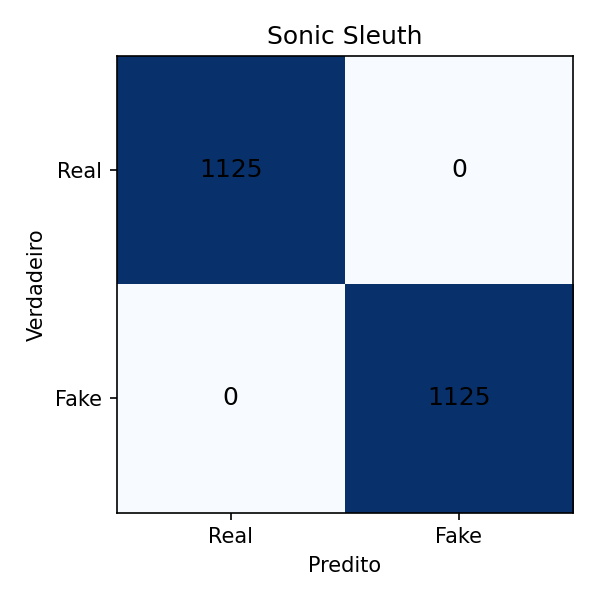
\includegraphics[width=\textwidth]{figures/confusion_matrices/sonic_sleuth.png}
        \caption{Sonic Sleuth}
    \end{subfigure}
    \hfill
    \begin{subfigure}[b]{0.32\textwidth}
        \centering
        
\includegraphics[width=\textwidth]{figures/confusion_matrices/aasist.png}
        \caption{AASIST}
    \end{subfigure}
    \hfill
    \begin{subfigure}[b]{0.32\textwidth}
        \centering
        
\includegraphics[width=\textwidth]{figures/confusion_matrices/rawgat_st.png}
        \caption{RawGAT-ST}
    \end{subfigure}

    \vspace{0.25cm}
    \begin{subfigure}[b]{0.32\textwidth}
        \centering
        
\includegraphics[width=\textwidth]{figures/confusion_matrices/conformer.png}
        \caption{Conformer}
    \end{subfigure}
    \hfill
    \begin{subfigure}[b]{0.32\textwidth}
        \centering
        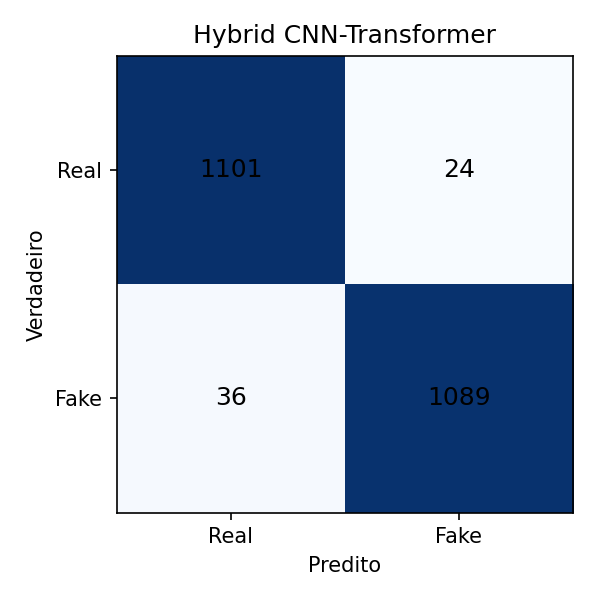
\includegraphics[width=\textwidth]{figures/confusion_matrices/hybrid_cnn_transformer.png}
        \caption{Hybrid CNN-Transformer}
    \end{subfigure}
    \hfill
    \begin{subfigure}[b]{0.32\textwidth}
        \centering
        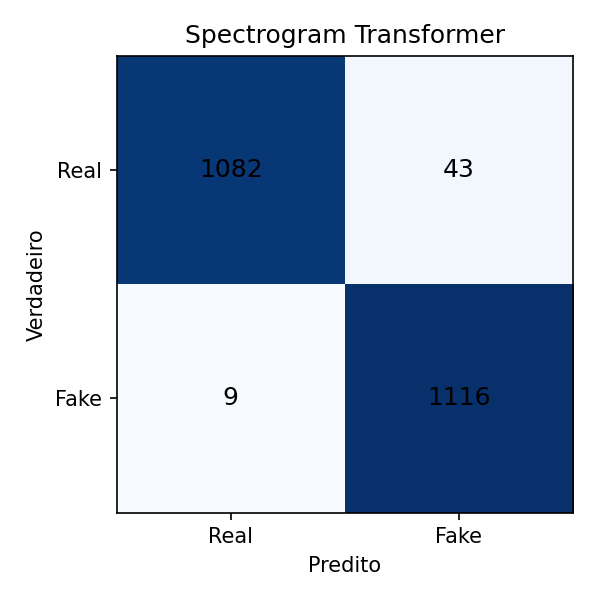
\includegraphics[width=\textwidth]{figures/confusion_matrices/spectrogram_transformer.png}
        \caption{Spectrogram Transformer}
    \end{subfigure}
    \caption{Matrizes de confusão, parte 1: SSL, raw-audio, grafos e Transformers.}
    \label{fig:confusion_all_neural_a}
\end{figure}

\begin{figure}[H]
    \centering
    \begin{subfigure}[b]{0.32\textwidth}
        \centering
        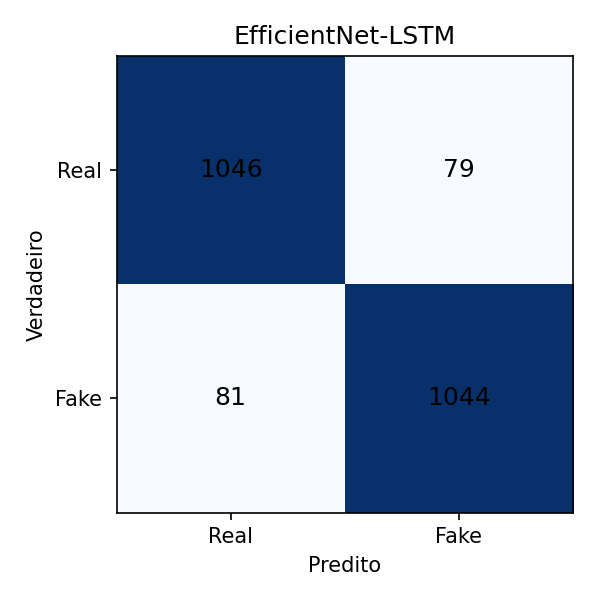
\includegraphics[width=\textwidth]{figures/confusion_matrices/efficientnet_lstm.png}
        \caption{EfficientNet-LSTM}
    \end{subfigure}
    \hfill
    \begin{subfigure}[b]{0.32\textwidth}
        \centering
        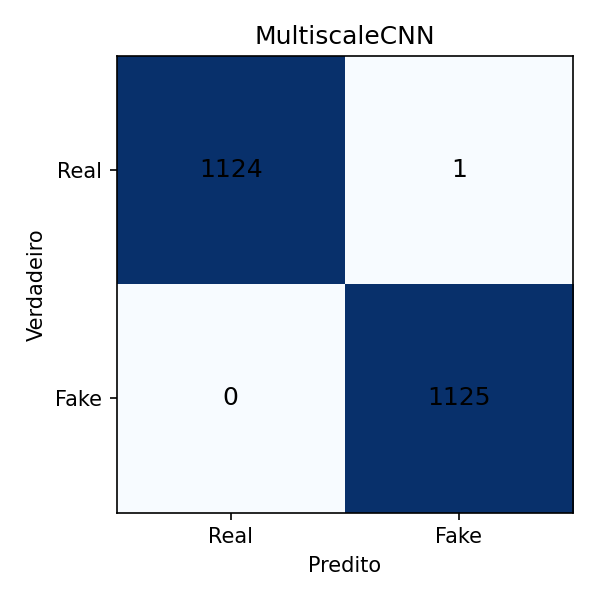
\includegraphics[width=\textwidth]{figures/confusion_matrices/multiscalecnn.png}
        \caption{MultiscaleCNN}
    \end{subfigure}
    \hfill
    \begin{subfigure}[b]{0.32\textwidth}
        \centering
        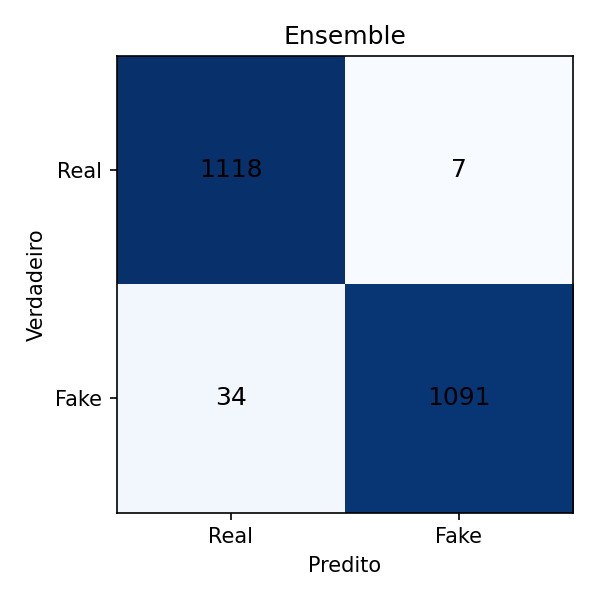
\includegraphics[width=\textwidth]{figures/confusion_matrices/ensemble.png}
        \caption{Ensemble}
    \end{subfigure}

    \vspace{0.25cm}
    \begin{subfigure}[b]{0.32\textwidth}
        \centering
        
\includegraphics[width=\textwidth]{figures/confusion_matrices/svm.png}
        \caption{SVM}
    \end{subfigure}
    \hfill
    \begin{subfigure}[b]{0.32\textwidth}
        \centering
        
\includegraphics[width=\textwidth]{figures/confusion_matrices/random_forest.png}
        \caption{Random Forest}
    \end{subfigure}
    \caption{Matrizes de confusão, parte 2: espectrais, Ensemble e linhas de base clássicas.}
    \label{fig:confusion_all_neural_b}
\end{figure}

\end{document}
